% 編譯方式：在 paper/ 目錄下執行  xelatex main.tex  （兩次，以更新目錄與參照）
%           或上傳整個專案至 Overleaf，編譯器選 XeLaTeX，主檔為 paper/main.tex
% 圖檔由 src/ 腳本產生於 ../outputs/figures/；請先執行 src/01~09。
\documentclass[UTF8,a4paper,11pt]{ctexart}
\usepackage[margin=2.5cm]{geometry}
\usepackage{graphicx,booktabs,caption,subcaption,amsmath,amssymb,hyperref,float,array}
\usepackage{xcolor}
\graphicspath{{../outputs/figures/}}
\captionsetup{font=small}
\hypersetup{colorlinks=true,linkcolor=blue!50!black,urlcolor=blue!50!black,citecolor=blue!50!black}
\setlength{\parindent}{2em}
\renewcommand{\arraystretch}{1.1}
\newcommand{\note}[1]{\textcolor{red!60!black}{【待確認：#1】}}

\title{台灣縣市肺癌發生與死亡之時空型態：\\主成分分析、分群與公共衛生意涵（1979--2022）}
\author{林\ \ \ \ \ \ \ \ 多變量分析期末報告}
\date{\today}

\begin{document}
\maketitle

\begin{abstract}
\noindent
肺癌是台灣癌症死亡之首，其疾病負擔在地理與時間上都並不均勻。本研究以1979至2022年21個縣市（排除連江縣）的肺癌年齡標準化發生率為對象，先以主成分分析（PCA）描繪縣市軌跡的主要結構，再以K-means、階層式分群及多種追蹤資料分群演算法歸併相似縣市，並以貝氏階層模型與空間約束分群分別處理小人口縣市的估計不穩與地理連續性問題；另結合衛生福利部死因統計，以死亡發生比（MIR）比較發生與死亡兩端指標。縣市平均發生率由1979年的每10萬人口9.6上升至2022年的39.8，縣市間變異係數則由0.61降至0.16，呈現「整體上升、差距收斂」。PCA顯示縣市之間存在長期穩定的空間梯度（北部都會與宜蘭偏高，苗栗、屏東、南投、新竹縣與金門偏低），以及早發的都會區與後發的中南部之間的時序翻轉。分群結果在K-means、Ward與高斯混合模型間高度一致，將縣市分為北部都會、中西部與南部偏鄉、其餘本島，以及金門、澎湖兩個小人口離島。貝氏階層模型顯示澎湖縣的高發生率部分來自小數個案的波動（2018--2022年由52.3收縮至46.3），但仍居全國最高；Moran's $I$則顯示發生率的空間群聚已由1979--83年的0.53消失，至2018--22年轉為$-0.24$。發生率與死亡率的縣市排序並不一致（2020--2022年相關係數0.33--0.53），屏東、台東與花蓮的死亡發生比偏高，提示診斷時期與醫療可近性的差異。文末討論研究限制，並對菸害防制、早期偵測與小區域監測提出建議。
\end{abstract}

\tableofcontents
\newpage

%=====================================================================
\section{緒論}
%=====================================================================
肺癌（ICD-10 C33--C34，氣管、支氣管及肺之惡性腫瘤）是台灣疾病負擔最重的癌症之一，其致病與診斷特性使它特別適合作為公共衛生監測的對象。首先，肺癌的潛伏期很長：從吸菸等暴露到發病，往往相隔二、三十年，因此今日的發生率反映的是數十年前的暴露，而今日菸害防制的成效，要等到未來才看得見。其次，肺癌早期症狀不明顯，多數個案確診時已是晚期，存活與否高度取決於診斷時的期別。這使得「發生」與「死亡」兩個指標雖然高度相關，卻會因為篩檢、診斷與治療的可近性而在不同地區拉開差距，只看其中一個指標，可能看不到另一端的問題。

台灣的肺癌圖像還有兩個值得留意的背景。男性長期是主要的吸菸族群，然而女性肺癌，尤其是肺腺癌，有相當比例發生在不吸菸者身上，提示二手菸、烹飪油煙、空氣污染與遺傳因素的重要性。同時，台灣在這四十餘年間歷經快速的工業化、都市化與人口老化，也經歷了菸害防制法（1997年制定、2009年大幅修正）與癌症防治法（2003年）等制度變遷\note{各法規之公布與施行日期請對照原條文}。肺癌的時空分布因此可以視為社會變遷與公共衛生政策的一扇長期觀察窗。

過去針對台灣死因地理差異的研究，多半討論全死因或主要死因的整體比較（楊敬賢等，2014；江信緯，2015；陳玟儒，2024）\note{請補齊完整書目}；對單一主要癌症、跨越四十餘年的縣市軌跡比較則相對少見。陳玟儒（2024）建議後續可嘗試K-means以外的分群演算法與不同死因，本文承接這個方向，除了加入階層式分群及其他追蹤資料常用的分群方法之外，還處理兩個實務上常被忽略的問題：小人口縣市的年度率值極不穩定，以及分群結果在地理上是否連續。最後，本文結合發生率與死亡率兩端指標，檢視兩者的地區排序是否一致。

具體而言，本文要回答下列問題：過去44年肺癌發生率在縣市間的水準與差距如何演變；縣市軌跡的主要變異結構為何，能否以空間梯度與時序型態解釋；縣市能否合理歸併為少數幾個可供借力估計與資源配置的參考群體，且此結論是否隨演算法而變；以及以發生率與以死亡率衡量的地區排序是否一致，不一致處又提示什麼樣的醫療與預防議題。

%=====================================================================
\section{資料與方法}
%=====================================================================
\subsection{資料與指標}
發生率取自癌症登記資料（\texttt{lung\_cancer\_incidence\_1979\_2022.csv}），選取癌別為「肺、支氣管及氣管」、性別為「全」，並排除「全國」列。指標為以WHO 2000世界標準人口（Ahmad et al., 2001）計算的年齡標準化發生率（ASIR，每10萬人口）：
\begin{equation}
\mathrm{ASIR}=\sum_{a} w_a\cdot r_a ,\qquad r_a=\frac{\text{年齡層 }a\text{ 之新診斷個案數}}{\text{年齡層 }a\text{ 之人年}}\times 10^5 ,
\end{equation}
其中 $w_a$ 為標準人口的年齡權重。年齡標準化消除了各縣市老化程度不同對粗率的干擾，使跨縣市與跨年度的比較成為可能。

死亡率取自衛生福利部死因統計的各縣市統計表（表2），選取C33--C34一列，取得合計及男、女別的年齡標準化死亡率（ASMR），標準人口同樣為WHO 2000。專案資料夾中可取得的年度為民國109至112年及114年，即西元2020至2023年與2025年；2024年（民國113年）的檔案不在資料夾中，因此發生率（至2022年）與死亡率重疊的年度僅有2020至2022年。我們以死亡發生比（mortality-to-incidence ratio, MIR）連結兩者：
\begin{equation}
\mathrm{MIR}_{c,t}=\frac{\mathrm{ASMR}_{c,t}}{\mathrm{ASIR}_{c,t}} .
\end{equation}
MIR常被當作癌症存活與照護成效的粗略代理指標，在其他條件相同下，MIR越高代表同樣的發生負擔轉為越多的死亡。但本文是以同一年的標準化率相除，並未追蹤同一世代，因此只能作為探索性的指標。

\subsection{前處理}
資料中的縣市別已採現行行政區劃，所以不需要另外對2010年縣市合併升格作加權合併，只需留意升格前後轄區範圍不同，早期發生率的解讀宜保守。連江縣人口極少，1979至2000年間有11個年度缺值（1979、1980、1981、1986、1989、1990、1992、1995、1997、1999與2000年），個案稀少又使比率劇烈跳動，為避免扭曲協方差結構而排除。金門與澎湖雖同為小人口離島，但序列完整，予以保留，並在結果中審慎詮釋。最後得到21個縣市乘以44個年度的矩陣。

\subsection{主成分分析}
我們將矩陣的每一欄（年度）在21個縣市之間標準化為平均0、標準差1，再對相關係數矩陣進行PCA，使各年度具有同等權重，避免變異較大的近期年度主導主成分的方向。需要特別強調的是，這個標準化同時移除了每一年度的全國平均水準，所以PCA描述的是縣市相對於同年度其他縣市的位置及其變化，而不是全國發生率的上升趨勢，後者另以描述統計呈現。縣市是圖上的點（得分），年度是箭頭（負荷量）；在相關係數矩陣PCA下，負荷量可直接解讀為該年度與主成分的相關係數。我們也計算只作欄中心化而不縮放的共變異數矩陣版本，作為穩健性檢查。

\subsection{分群方法}
分群的對象是標準化後的縣市軌跡。主分析使用K-means（$k=2,\dots,10$，隨機種子固定）與階層式分群（歐氏距離，single、complete、average與Ward連結），以肘部法與輪廓係數（Rousseeuw, 1987）協助選擇群數。為檢驗結論是否取決於演算法，我們另納入追蹤資料分群中常見的幾個家族：以實際縣市為中心的K-medoids（PAM），對離群軌跡較不敏感；以$1-r$為距離、只比較軌跡形狀的相關係數階層式分群；允許軌跡在時間軸上小幅位移的動態時間校正（DTW）距離，搭配階層式與K-medoids；以5-近鄰圖為親和矩陣的譜分群；以及模型式分群，包括對前4個主成分得分配適的高斯混合模型（GMM，以BIC選群數），和對每個縣市二次趨勢的水準、斜率與曲率三個係數配適的GMM，後者可視為潛在類別成長模型的簡化替代。此外還有給出隸屬度的模糊C平均，以及能將不屬於任何密集群體之軌跡標為雜訊的DBSCAN。各方法與Ward分群的一致性以調整後蘭德指數（ARI，1為完全一致，0約為隨機）衡量，穩定性則以對年度欄位重抽樣（100次，每次重新標準化與分群）後與原分群的平均ARI衡量。

\subsection{貝氏階層模型}\label{sec:bayes}
小人口縣市的年度個案數很少，直接比較原始標準化率容易把隨機波動誤認為真實差異。我們因此以貝氏階層模型（部分合併）估計各縣市的長期軌跡。令 $y_{ct}=\log \mathrm{ASIR}_{ct}$，並以登記個案數 $n_{ct}$ 搭配delta法近似其抽樣變異 $\mathrm{Var}(y_{ct})\approx\phi/n_{ct}$，其中 $\phi$ 是吸收年齡標準化加權所增加之變異的過度離散參數：
\begin{align}
y_{ct}\mid\boldsymbol\theta_c,\phi &\sim N\!\left(\mathbf x_t^{\top}\boldsymbol\theta_c,\ \phi/n_{ct}\right), & \mathbf x_t&=(1,\tau_t,\tau_t^2),\\
\boldsymbol\theta_c\mid\boldsymbol\mu,\Sigma &\sim N_3(\boldsymbol\mu,\Sigma), & \boldsymbol\mu&\sim N_3(0,10^2 I),\\
\Sigma&\sim \text{Inv-Wishart}(\nu_0,\Psi_0), & \phi&\sim \text{Inv-Gamma}(0.01,0.01).
\end{align}
這裡 $\tau_t$ 是標準化後的年度，$\boldsymbol\theta_c$ 是縣市 $c$ 的水準、斜率與曲率。所有全條件分配皆為共軛，故以Gibbs抽樣估計（6000次迭代，捨棄前1500次，每5次保留1次，共900筆後驗樣本）。此模型使個案數少的縣市向全體平均收縮，並給出每個縣市水準、排名與趨勢的可信區間。為使分群也反映不確定性，我們另對300筆後驗樣本的 $\boldsymbol\theta$ 各做一次 $k=5$ 的K-means，統計縣市兩兩被分在同一群的後驗機率。

\subsection{空間約束分群與空間自相關}\label{sec:spatial}
一般分群只依軌跡相似度合併，群內縣市不一定在地理上相連，但公共衛生上的「區域」通常要求地理連續。因此我們另做空間約束的Ward階層式分群：以縣市界線建立queen鄰接圖（共邊或共點即相鄰），兩群只有在含有相鄰縣市時才可合併。澎湖與金門沒有陸地邊界，我們把它們各連到距離最近的兩個縣市（澎湖連至嘉義縣與雲林縣，金門連至台中市與澎湖縣），這是為保持鄰接圖連通而作的人為設定，結果對此設定有一定依賴。我們並以全域Moran's $I$（列標準化權重，9999次置換檢定）檢驗發生率與PCA得分的空間自相關：
\begin{equation}
I=\frac{n}{\sum_{i,j}w_{ij}}\cdot\frac{\sum_{i,j}w_{ij}(x_i-\bar x)(x_j-\bar x)}{\sum_i (x_i-\bar x)^2}.
\end{equation}

%=====================================================================
\section{結果}
%=====================================================================
\subsection{全國趨勢與縣市差距的收斂}\label{sec:trend}
21個縣市（未加權）平均的發生率由1979年的9.6上升至1989年的19.0、1999年的27.9與2009年的33.6，2019年達40.1，2022年為39.8（每10萬人口）；上升在2010年代前半趨緩（2009年33.6、2014年34.2），其後再度上揚。與此同時，縣市間的相對離散大幅縮小，變異係數由1979年的0.61降至1989年的0.24、1999年的0.23、2009年的0.18與2022年的0.16。肺癌發生率因此經歷了水準大幅墊高、地區差距相對收斂的過程。早期的高離散一部分反映真實的區域差異（都會區較早進入高發階段），另一部分則可能來自早年各地登記完整性不一與小數個案造成的隨機波動。

\begin{figure}[H]
  \centering
  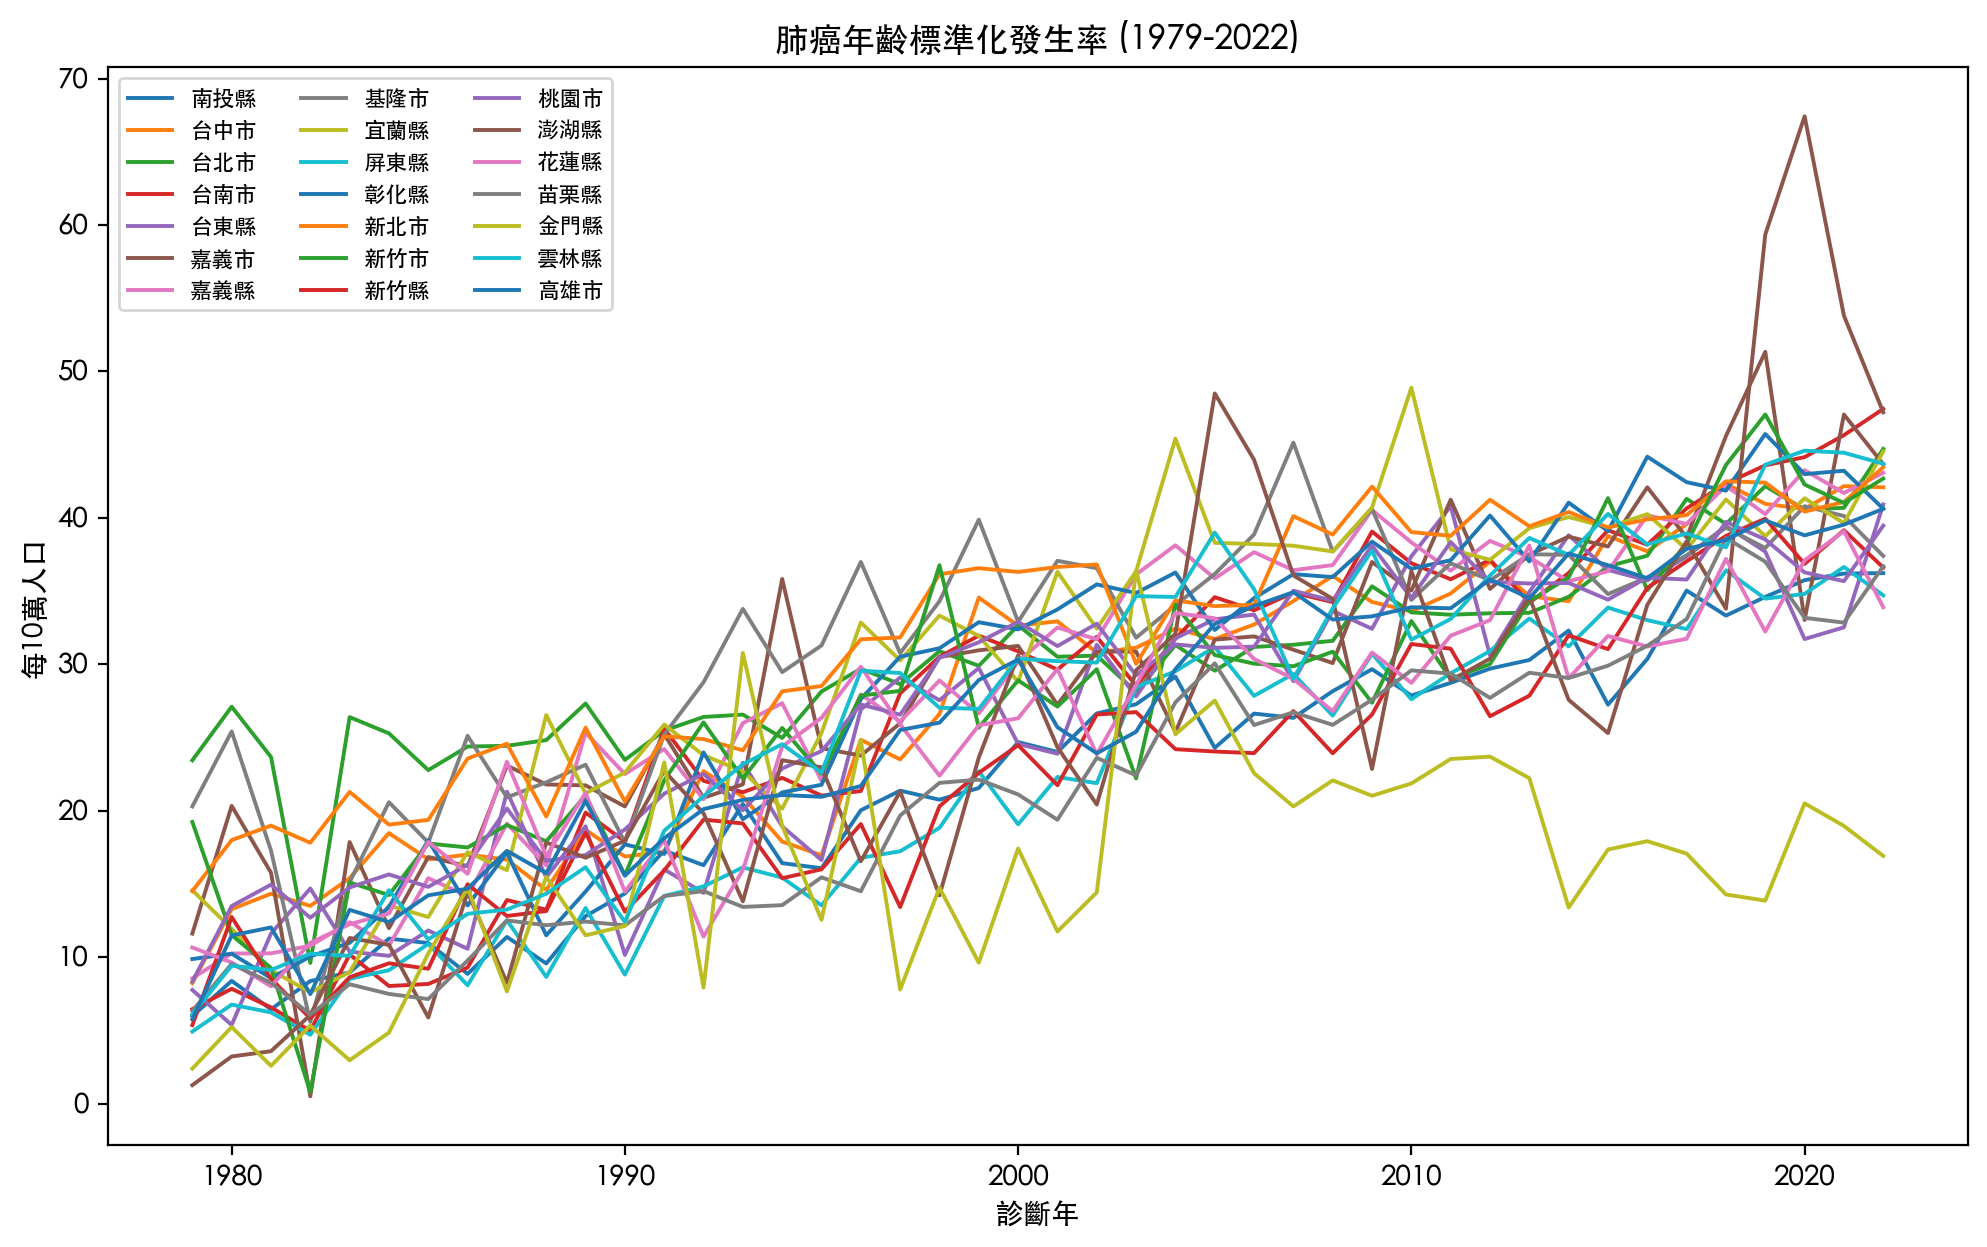
\includegraphics[width=.92\textwidth]{eda_trend_lines.png}
  \caption{各縣市肺癌年齡標準化發生率（1979--2022）。}\label{fig:trend}
\end{figure}

比較1979--1983與2018--2022兩個五年平均（附錄表\ref{tab:counties}），軌跡大致可分為三種類型。北部都會區起點最高而倍數最小：台北市由22.0增至41.5（1.9倍），新北市由18.1增至42.0（2.3倍），基隆市由16.7增至39.1（2.3倍），絕對增加量在本島中最低（台北市$+19.5$）。中南部則是後發而追趕：台南市由7.2增至44.6（6.2倍，增加$+37.4$），雲林縣（$+33.9$）、彰化縣（$+32.9$）與新竹市（$+32.1$）亦增加幅度大。離島則呈現極端：澎湖縣由5.1升至52.3（約10倍），為全國最高，金門縣僅由3.7升至16.9，為全國最低。

\subsection{主成分分析：空間梯度與時序翻轉}
相關係數矩陣PCA的前七個主成分解釋變異依序為53.6\%、13.6\%、8.2\%、6.9\%、3.4\%、2.6\%與2.5\%，累積分別為53.6\%、67.2\%、75.4\%、82.3\%、85.7\%、88.3\%與90.8\%；共變異數矩陣版本相近（PC1為54.1\%、PC2為16.0\%、前四個累積84.6\%），顯示結論對縮放方式不敏感。陡坡圖在第3至4個主成分之後趨於平坦（圖\ref{fig:scree}），以前2至4個主成分描述資料結構是合理的。

\begin{figure}[H]
  \centering
  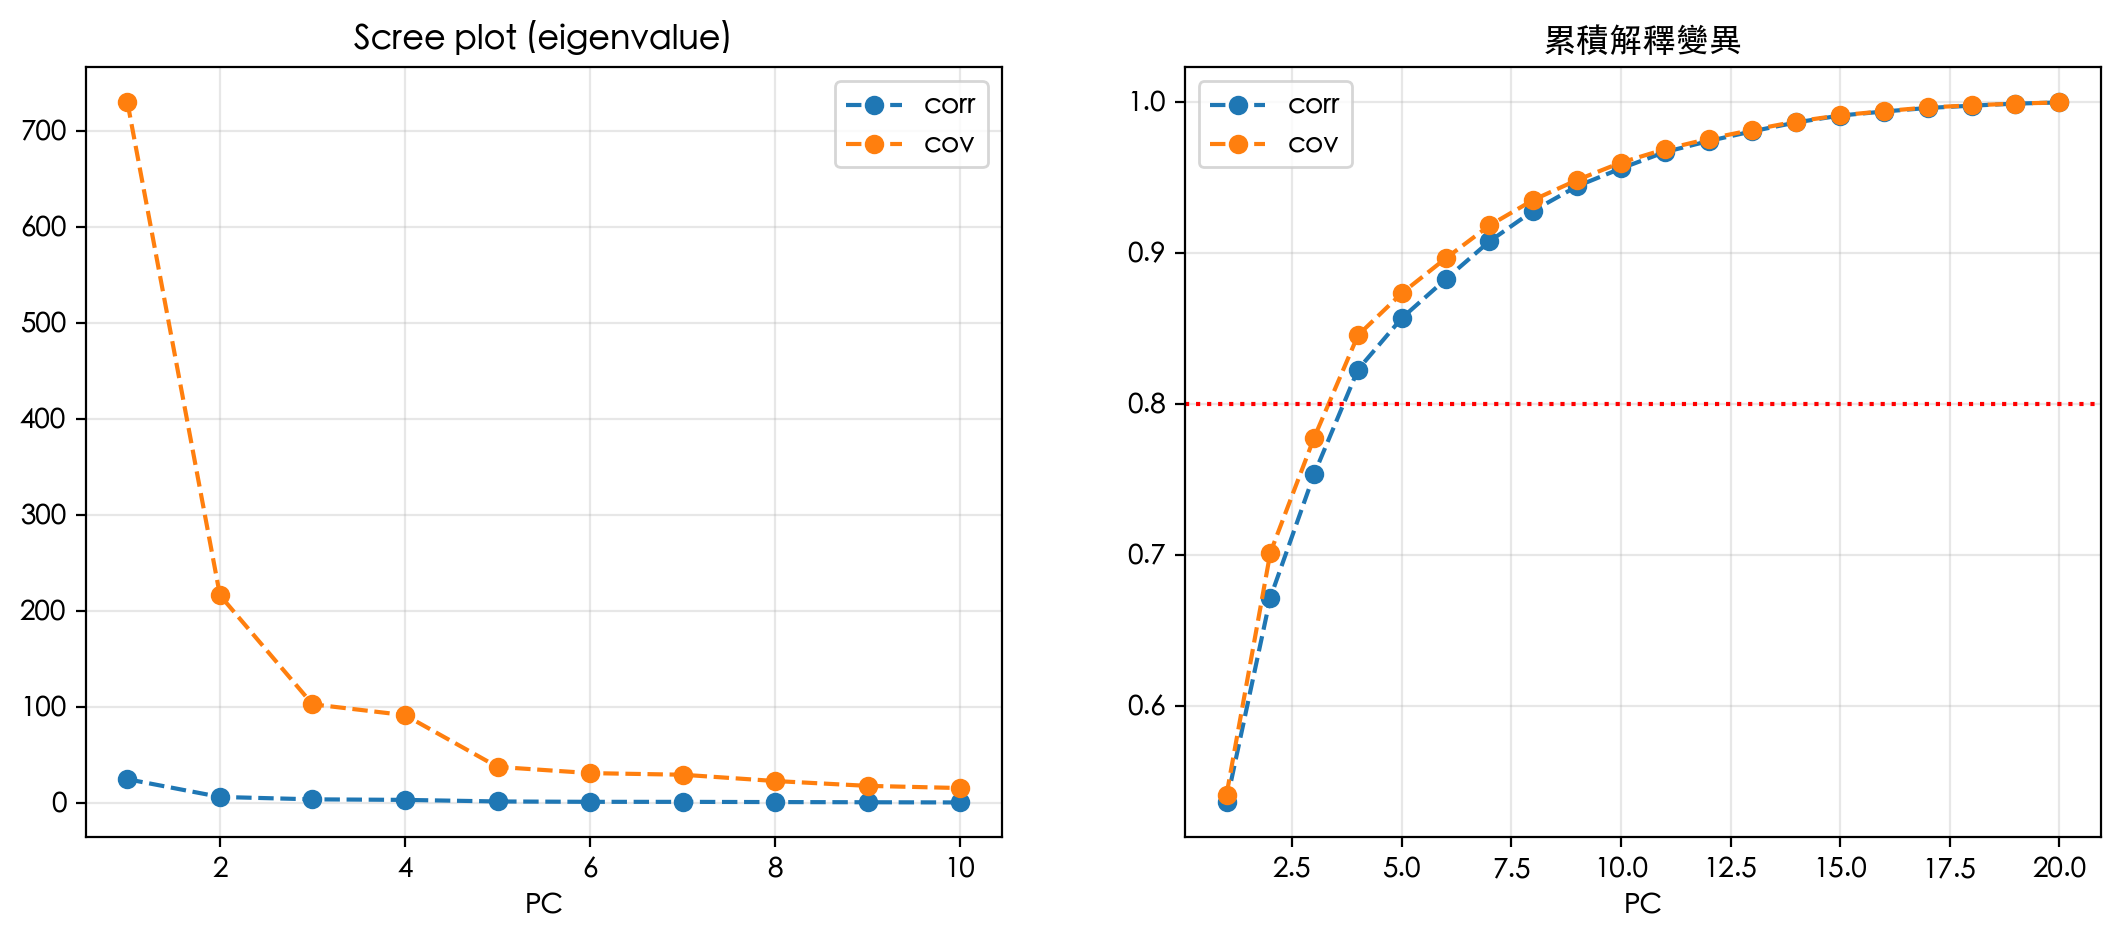
\includegraphics[width=.9\textwidth]{pca_scree_cumulative.png}
  \caption{陡坡圖與累積解釋變異（相關係數矩陣與共變異數矩陣）。}\label{fig:scree}
\end{figure}

第一主成分在全部44個年度上的負荷量都是正的（0.59至0.93，例如1999年0.93、2009年0.86、2022年0.77），表示它捕捉的是縣市在各年度大致維持相同相對位置這個共同結構。縣市得分顯示，新北市（$+7.2$）、基隆市（$+6.3$）、台北市（$+5.2$）、宜蘭縣（$+4.9$）以及嘉義市與嘉義縣（約$+3.3$）長期相對偏高，金門縣（$-13.2$）、苗栗縣（$-6.5$）、屏東縣（$-6.1$）、南投縣（$-5.3$）與新竹縣（$-5.1$）則長期相對偏低。縣市兩兩之間的Pearson相關係數中位數為0.88，本島主要縣市多落在0.8至0.99之間，金門與本島縣市的相關最低（與台北市僅0.36）。必須強調的是，PC1因此是一個持久的地理不平等，而不是時間趨勢。北部都會與宜蘭長期偏高，常被認為與較早都市化、較早採行西化生活型態及較早的吸菸盛行有關；苗栗、屏東、南投、新竹縣與金門長期偏低，則可能與吸菸史與人口組成的差異、早期診斷與登記完整性的差異，以及人口流動造成的就醫地與戶籍地不同有關。由於本文採用生態學資料，這些都只是有待檢驗的假說。

第二主成分呈現了時序上的翻轉。其負荷量在1979至1996年多為正（0.2至0.7），1997至2003年在0附近，2004年之後轉為負，2019至2022年約為$-0.55$至$-0.67$。對應的縣市得分是：台北市（$+4.7$）、基隆市（$+3.4$）、新北市（$+1.8$）與金門縣（$+5.4$）為正，也就是早期相對偏高、近期被追平甚至偏低；澎湖縣（$-5.7$）、台南市（$-3.0$）、彰化縣（$-2.1$）與雲林縣（$-2.0$）為負，也就是早期相對偏低、近期相對偏高（圖\ref{fig:biplot}）。這與前一節的追趕現象吻合，也呼應流行病學轉型的典型圖像：高發生率先出現在都會區，之後隨吸菸行為、工業與交通污染暴露、生活型態在全島擴散與人口老化，中南部迅速趕上。符號轉換的時間約在1997至2003年，與菸害防制法制定（1997）、癌症防治法（2003）及癌症登記品質提升的時期相近，但本資料無法區分這些因素，不宜作因果主張。

\begin{figure}[H]
  \centering
  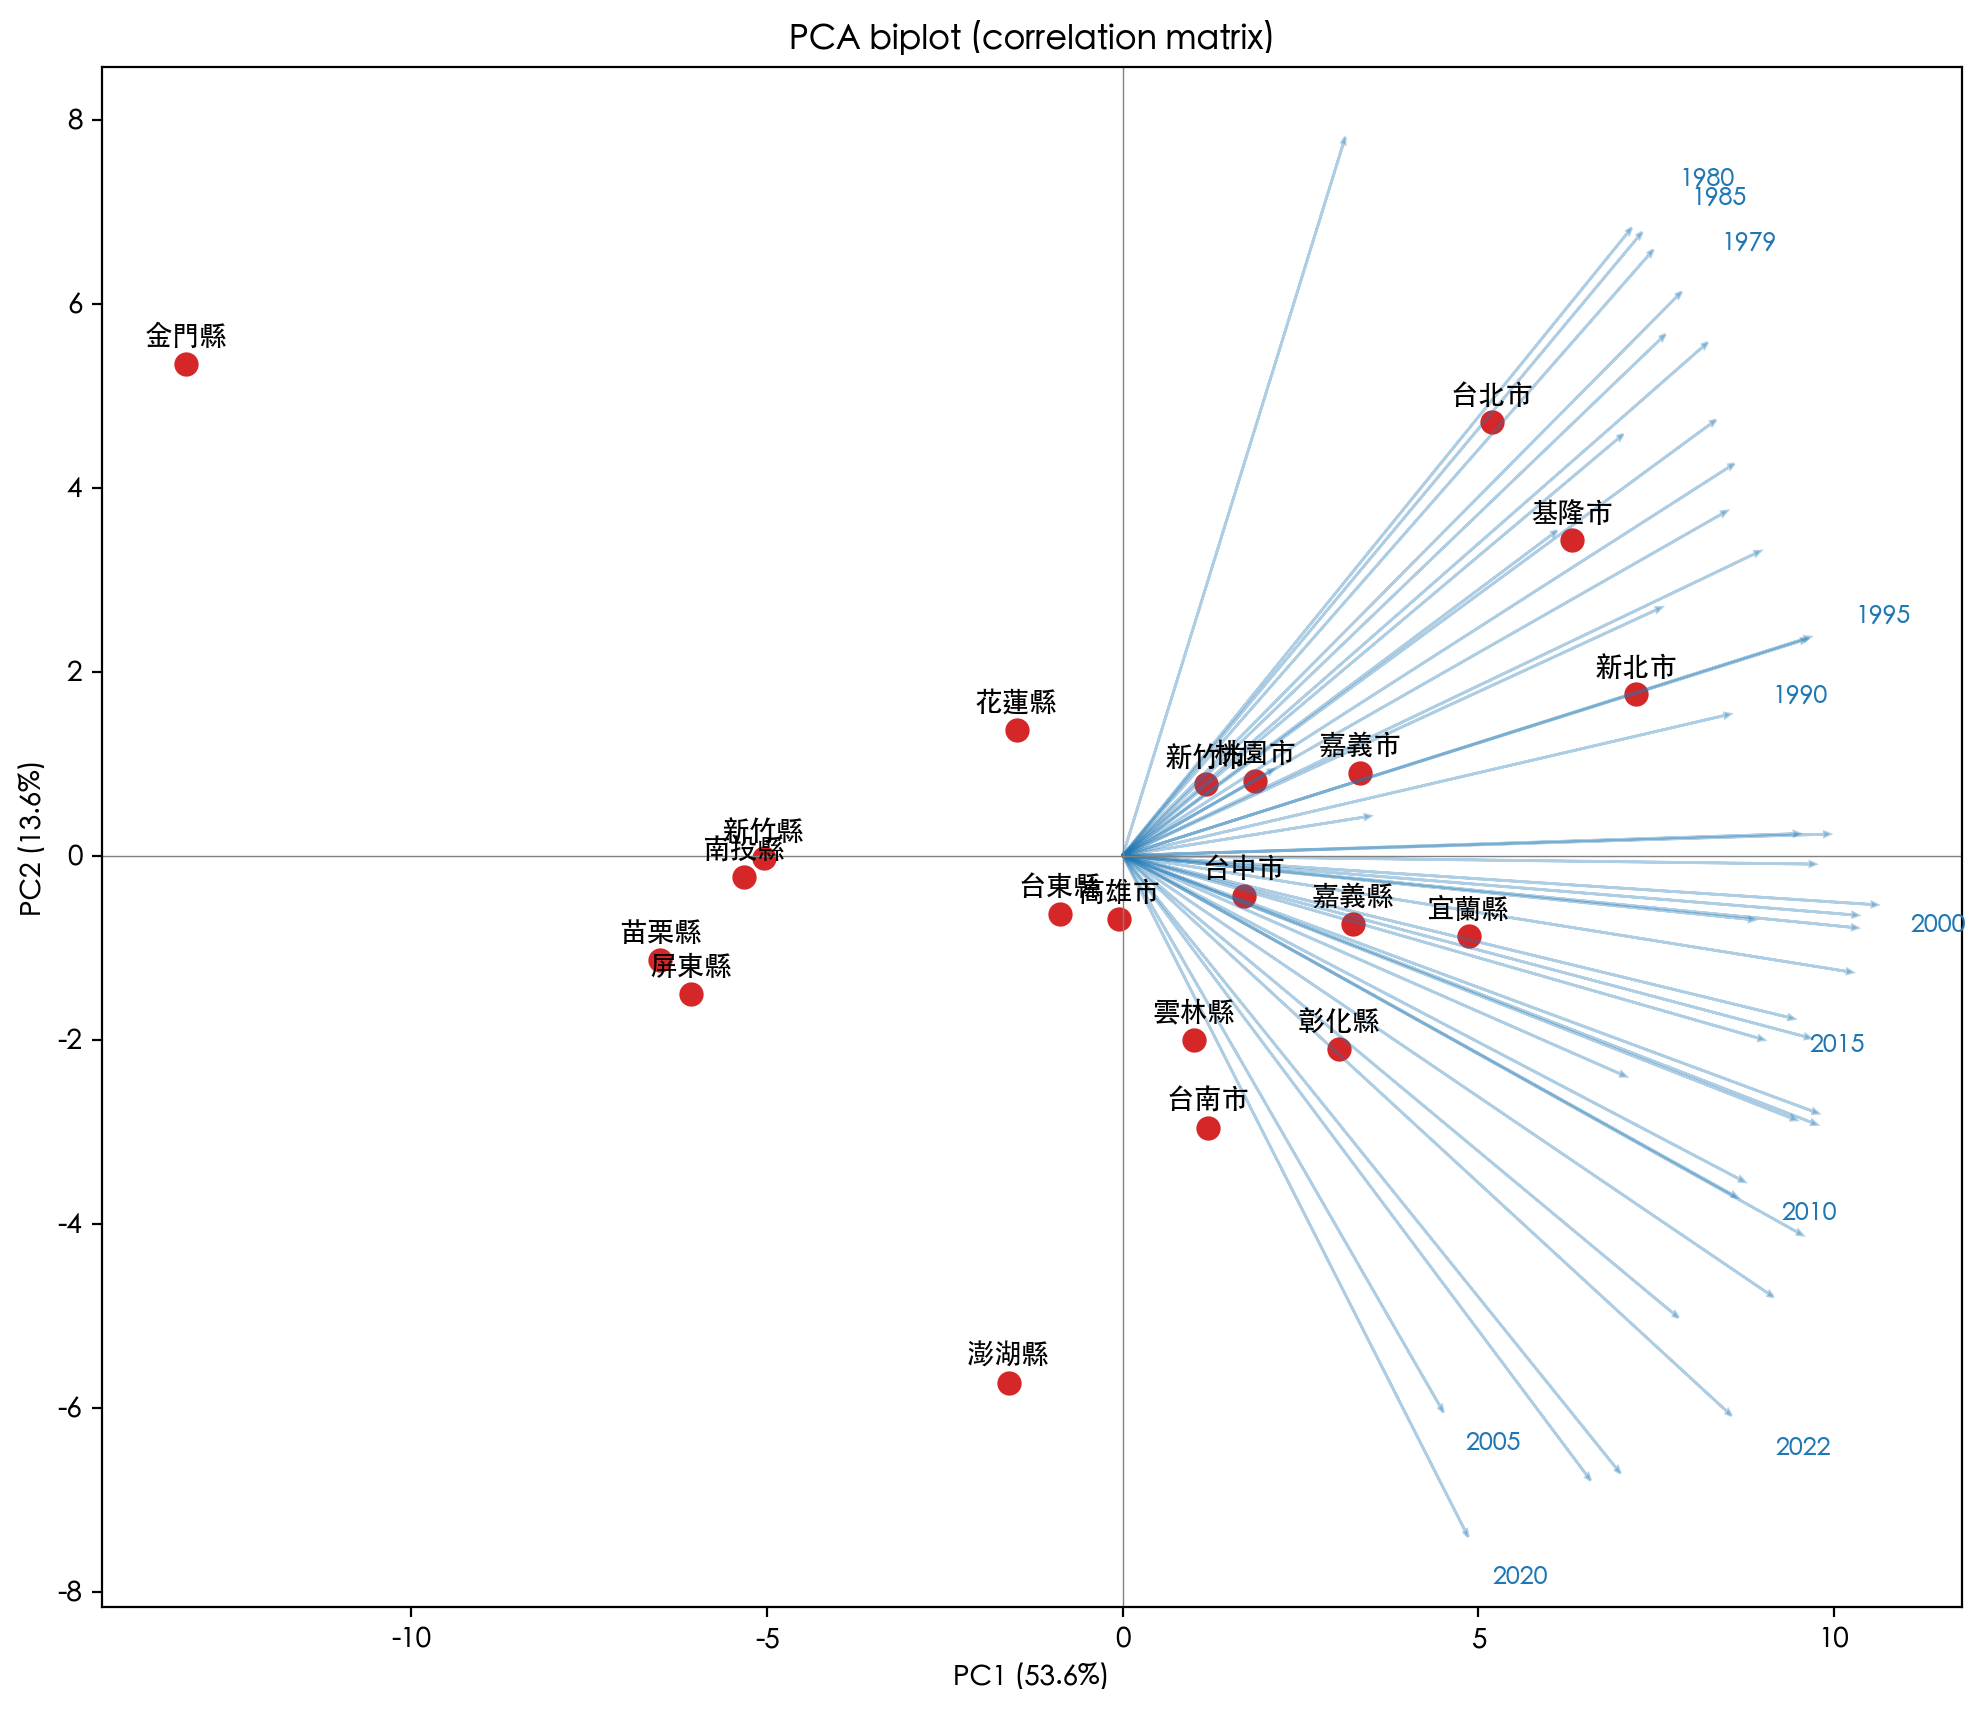
\includegraphics[width=.78\textwidth]{pca_biplot_corr.png}
  \caption{PCA雙標圖（相關係數矩陣）：點為縣市，箭頭為年度（標示每5年）。}\label{fig:biplot}
\end{figure}

第三與第四主成分（各解釋8.2\%與6.9\%）最極端的得分來自澎湖縣（PC3 $+4.3$、PC4 $-4.2$）與金門縣（PC3 $+4.0$）。PC4在2019至2021年的負荷量約為$-0.4$至$-0.5$，而同期澎湖縣的發生率由2018年的33.8躍升至2019年的59.4與2020年的67.4，再回落至2021年的53.8與2022年的47.2。這樣高度局部化的波動，較合理的解釋是小人口縣市因個案數少而產生的隨機變異（澎湖每年死亡個案僅約50至60人），而不宜直接歸因於COVID-19。若要評估疫情對診斷的影響，需要以月別或期別資料搭配全國層級模型另行分析。\note{原稿曾將PC4與疫情連結，此處改為保守說法，請確認或補充佐證}

\subsection{分群：核心結構與演算法的穩健性}
群數的選擇並無單一明確答案。K-means的輪廓係數在 $k=2$ 最高（0.349），$k=5$ 次之（0.252），$k=3$ 為0.244、$k=4$ 為0.225，SSE在 $k=2$ 至5間持續下降（574.7、464.0、359.0、281.7），沒有明顯的單一肘點（圖\ref{fig:select}）。階層式分群的 $k=2$ 以single、complete與average連結得到較高的輪廓係數（0.461，Ward為0.349），但檢視分群內容可知，這三種方法都只是把金門縣單獨切出、其餘20縣市為同一群，較高的輪廓係數來自離群點被孤立，並非更好的區域劃分。相對地，K-means與Ward在 $k=2$ 給出相同且較有公共衛生意義的分割：南投、屏東、新竹縣、苗栗與金門為長期相對偏低的一群，其餘16縣市為另一群。

\begin{figure}[H]
  \centering
  \begin{subfigure}{.49\textwidth}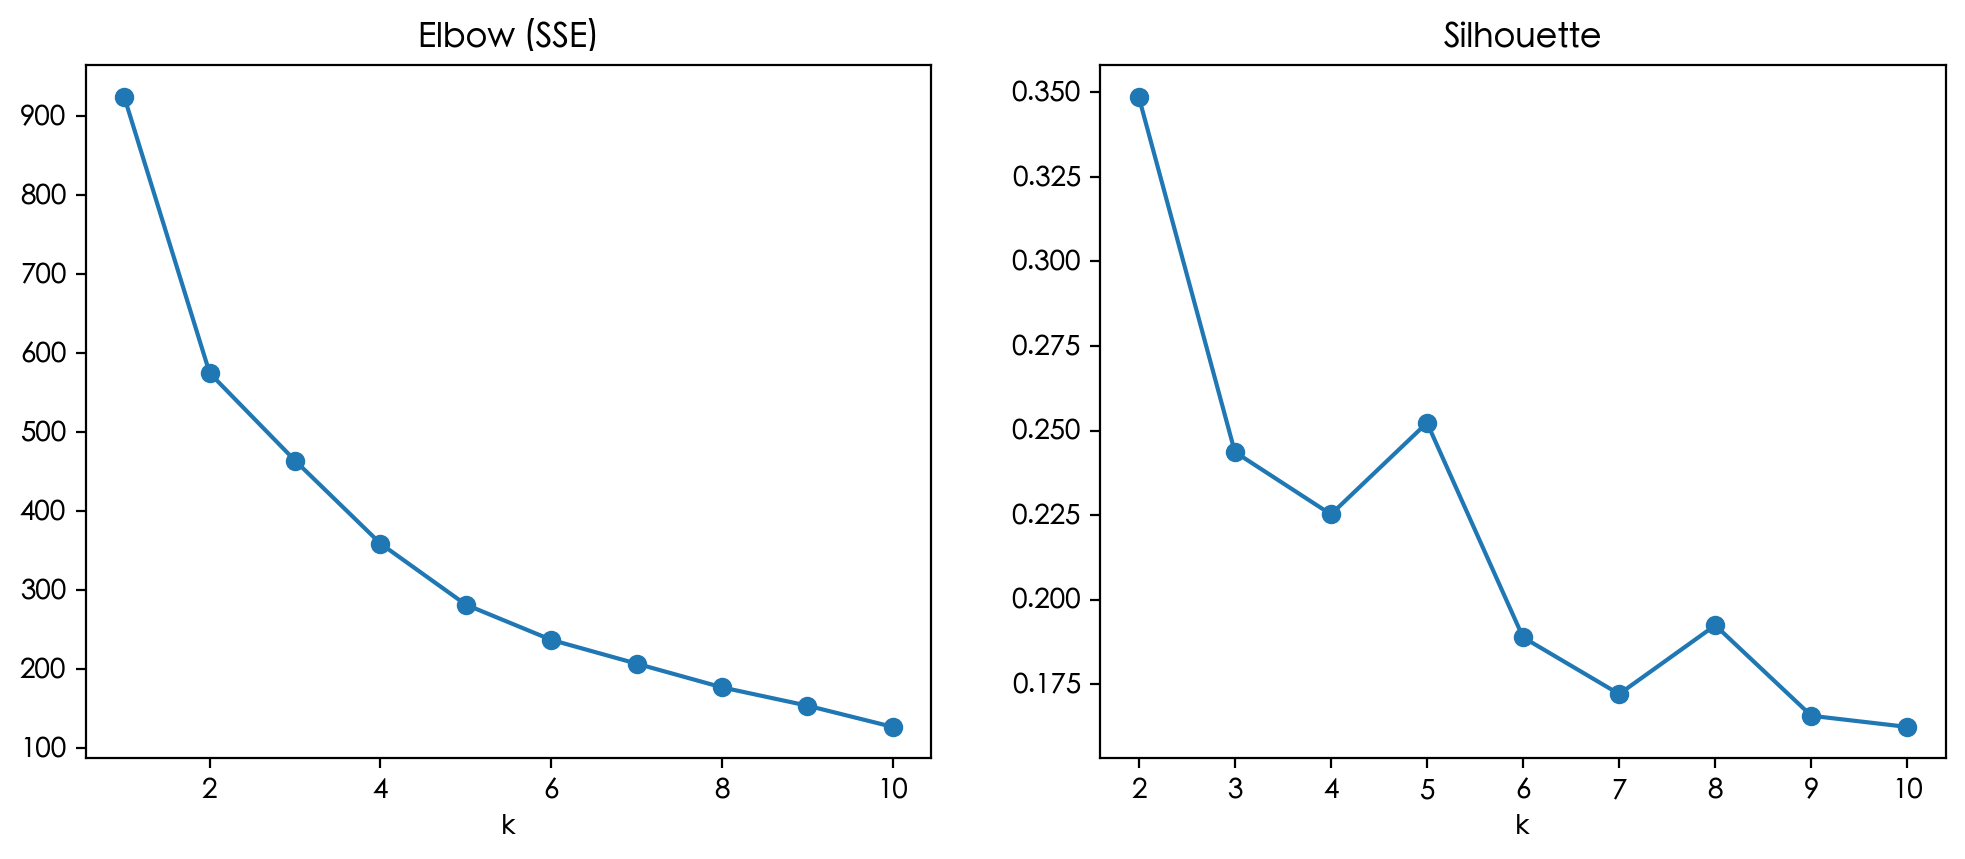
\includegraphics[width=\textwidth]{kmeans_elbow_silhouette.png}\caption{K-means之肘部與輪廓係數}\end{subfigure}
  \begin{subfigure}{.49\textwidth}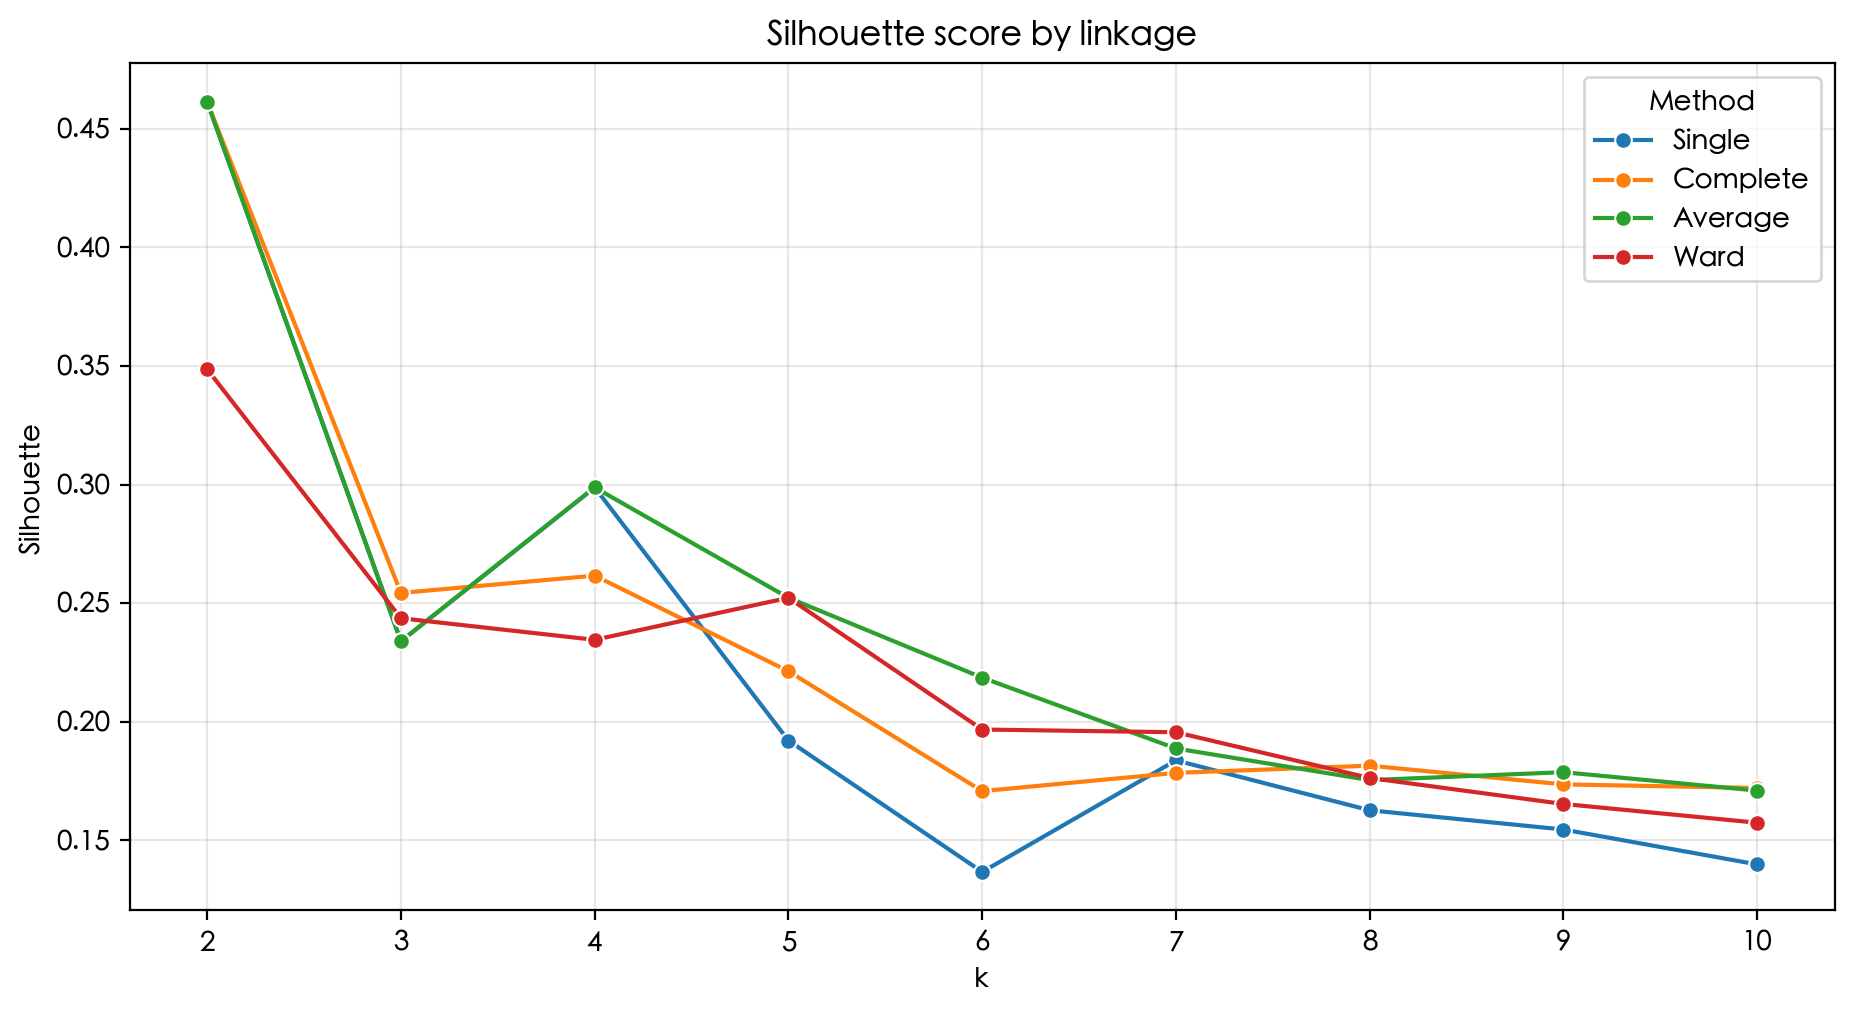
\includegraphics[width=\textwidth]{hclust_silhouette.png}\caption{階層式分群之輪廓係數}\end{subfigure}
  \caption{群數選擇。}\label{fig:select}
\end{figure}

在 $k=5$，K-means與Ward的成員完全一致，且各群的平均軌跡具有清楚的公共衛生語意（表\ref{tab:clusters}，圖\ref{fig:wardmap}）。北部都會群（台北、基隆、新北）與中西部南部偏鄉群（南投、屏東、新竹縣、苗栗）在早期相差約11.6，至近期縮小為約4.8；北部都會群與佔12個縣市的「其餘本島」群在近期幾乎重疊（40.9對41.0），顯示地區差距已大幅收斂。澎湖與金門因人口基數小、年度波動大，被各自獨立成群；這是統計上穩定的表現，不宜過度解讀為特殊的環境暴露。$k=4$的K-means則把宜蘭併入北部都會群，說明宜蘭位於都會群與其餘本島群的邊界。

\begin{table}[H]
\centering
\caption{$k=5$分群（K-means與Ward一致）及群內縣市平均之發生率（每10萬人口）。}\label{tab:clusters}
\small
\begin{tabular}{l p{6.4cm} cc}
\toprule
群 & 成員 & 1979--83 & 2018--22\\
\midrule
北部都會群 & 台北市、基隆市、新北市 & 19.0 & 40.9\\
其餘本島（12縣市） & 台中市、台南市、台東縣、嘉義市、嘉義縣、宜蘭縣、彰化縣、新竹市、桃園市、花蓮縣、雲林縣、高雄市 & 10.6 & 41.0\\
中西部與南部偏鄉群 & 南投縣、屏東縣、新竹縣、苗栗縣 & 7.4 & 36.1\\
澎湖 & 澎湖縣 & 5.1 & 52.3\\
金門 & 金門縣 & 3.7 & 16.9\\
\bottomrule
\end{tabular}
\end{table}

\begin{figure}[H]
  \centering
  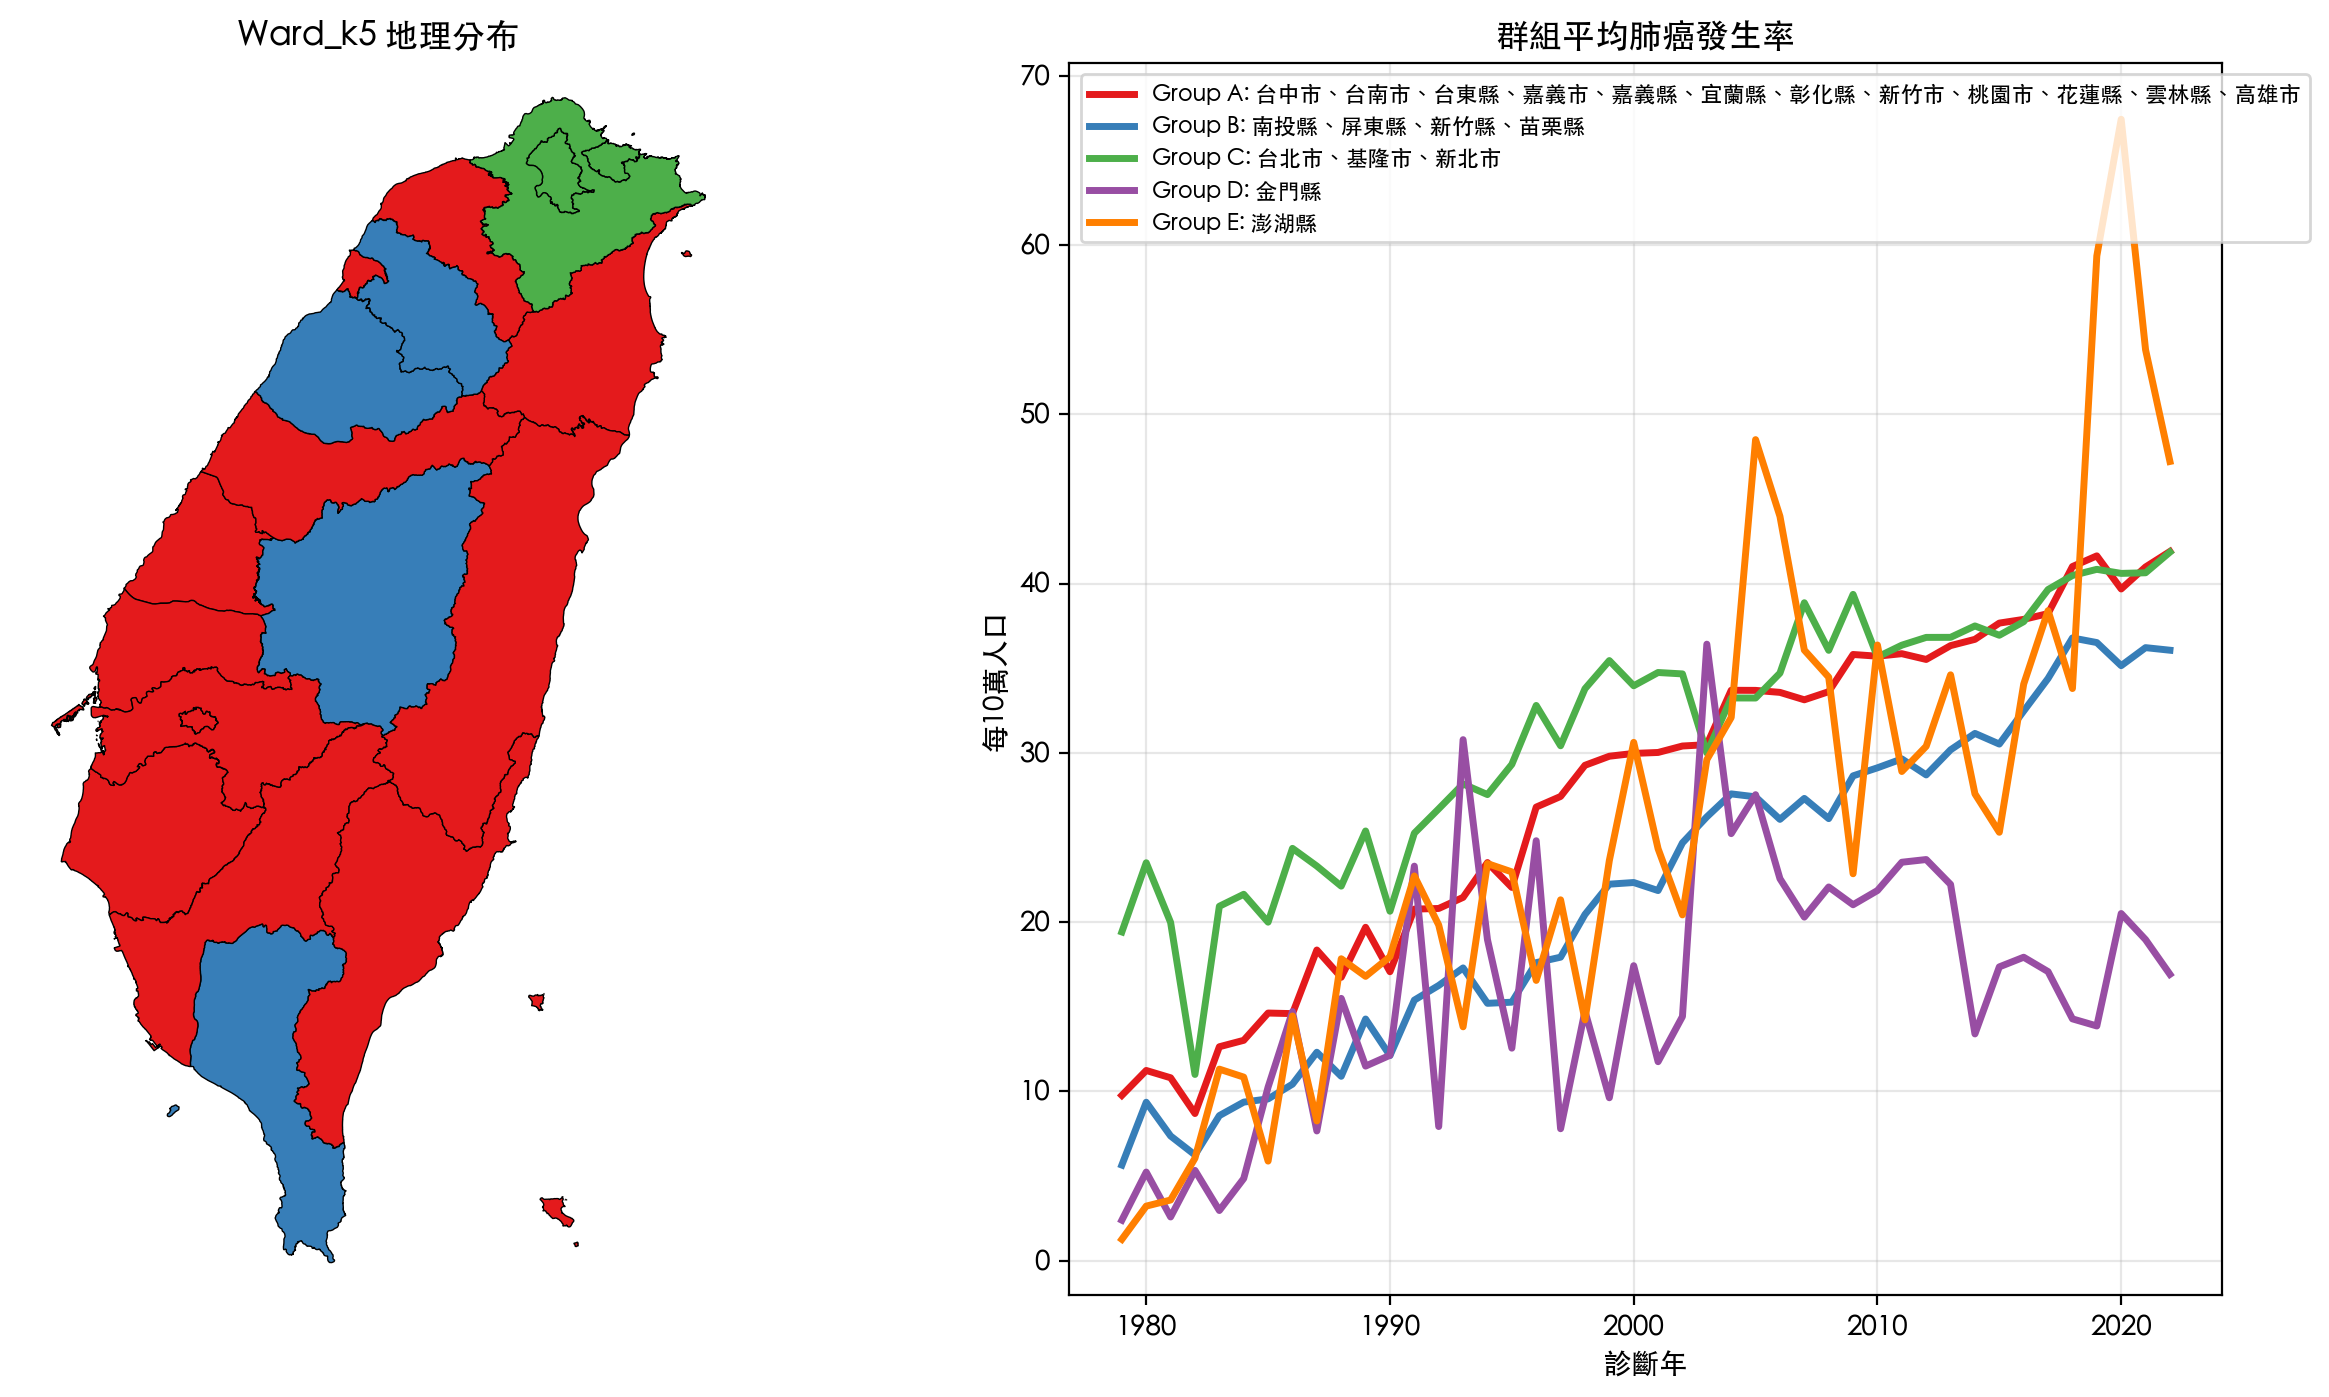
\includegraphics[width=\textwidth]{map_trend_Ward_k5.png}
  \caption{Ward法 $k=5$ 之縣市分群地圖（左）與各群平均軌跡（右）；K-means $k=5$ 之結果相同。}\label{fig:wardmap}
\end{figure}

這個核心分割並非某個演算法的產物。表\ref{tab:ari}顯示，K-means、Ward與對前4個主成分得分配適的GMM在 $k=5$ 給出完全相同的分割（ARI $=1.00$），DTW階層式與歐氏PAM的ARI為0.85，差別只在宜蘭縣被併入北部都會群。年度重抽樣下，Ward（平均ARI 0.79）、GMM（0.79）與K-means（0.72）最穩定；PAM（0.56）與譜分群（0.58）在 $k=5$ 較不穩定，且譜分群將嘉義市、新竹市、台南市與彰化縣等劃進不同於主分割的群，反映這些縣市位於群與群的邊界。$k=2$的分割更為穩健：K-means、Ward、譜分群與DTW-PAM給出相同的二分（ARI $=1.00$），年度重抽樣的平均ARI為0.82至0.88，是各 $k$ 中最穩定者。

\begin{table}[H]
\centering
\caption{各分群演算法與Ward分群之一致性（ARI），及年度重抽樣之穩定性（平均ARI，100次）。「--」表示未計算。}\label{tab:ari}
\small
\begin{tabular}{lcccc|cc}
\toprule
 & \multicolumn{4}{c|}{ARI vs.\ Ward} & \multicolumn{2}{c}{Bootstrap ARI}\\
演算法 & $k=2$ & $k=3$ & $k=4$ & $k=5$ & $k=2$ & $k=5$\\
\midrule
K-means & 1.00 & 1.00 & 0.85 & 1.00 & 0.82 & 0.72\\
Ward & 1.00 & 1.00 & 1.00 & 1.00 & 0.88 & 0.79\\
GMM（PCA得分） & 0.80 & 0.60 & 1.00 & 1.00 & 0.81 & 0.79\\
PAM（歐氏） & 0.80 & 0.47 & 0.55 & 0.85 & 0.84 & 0.56\\
譜分群（kNN） & 1.00 & 1.00 & 0.54 & 0.40 & 0.87 & 0.58\\
階層式（DTW, average） & 0.20 & 0.60 & 0.55 & 0.85 & -- & --\\
PAM（DTW） & 1.00 & 0.85 & 0.70 & 0.55 & -- & --\\
GMM（成長曲線係數） & 0.20 & 0.07 & 0.74 & 0.42 & -- & --\\
模糊C平均 & 0.63 & 0.61 & 0.35 & 0.44 & -- & --\\
階層式（相關係數距離, average） & $-0.04$ & 0.03 & 0.09 & $-0.01$ & 0.28 & 0.39\\
\bottomrule
\end{tabular}
\end{table}

\begin{figure}[H]
  \centering
  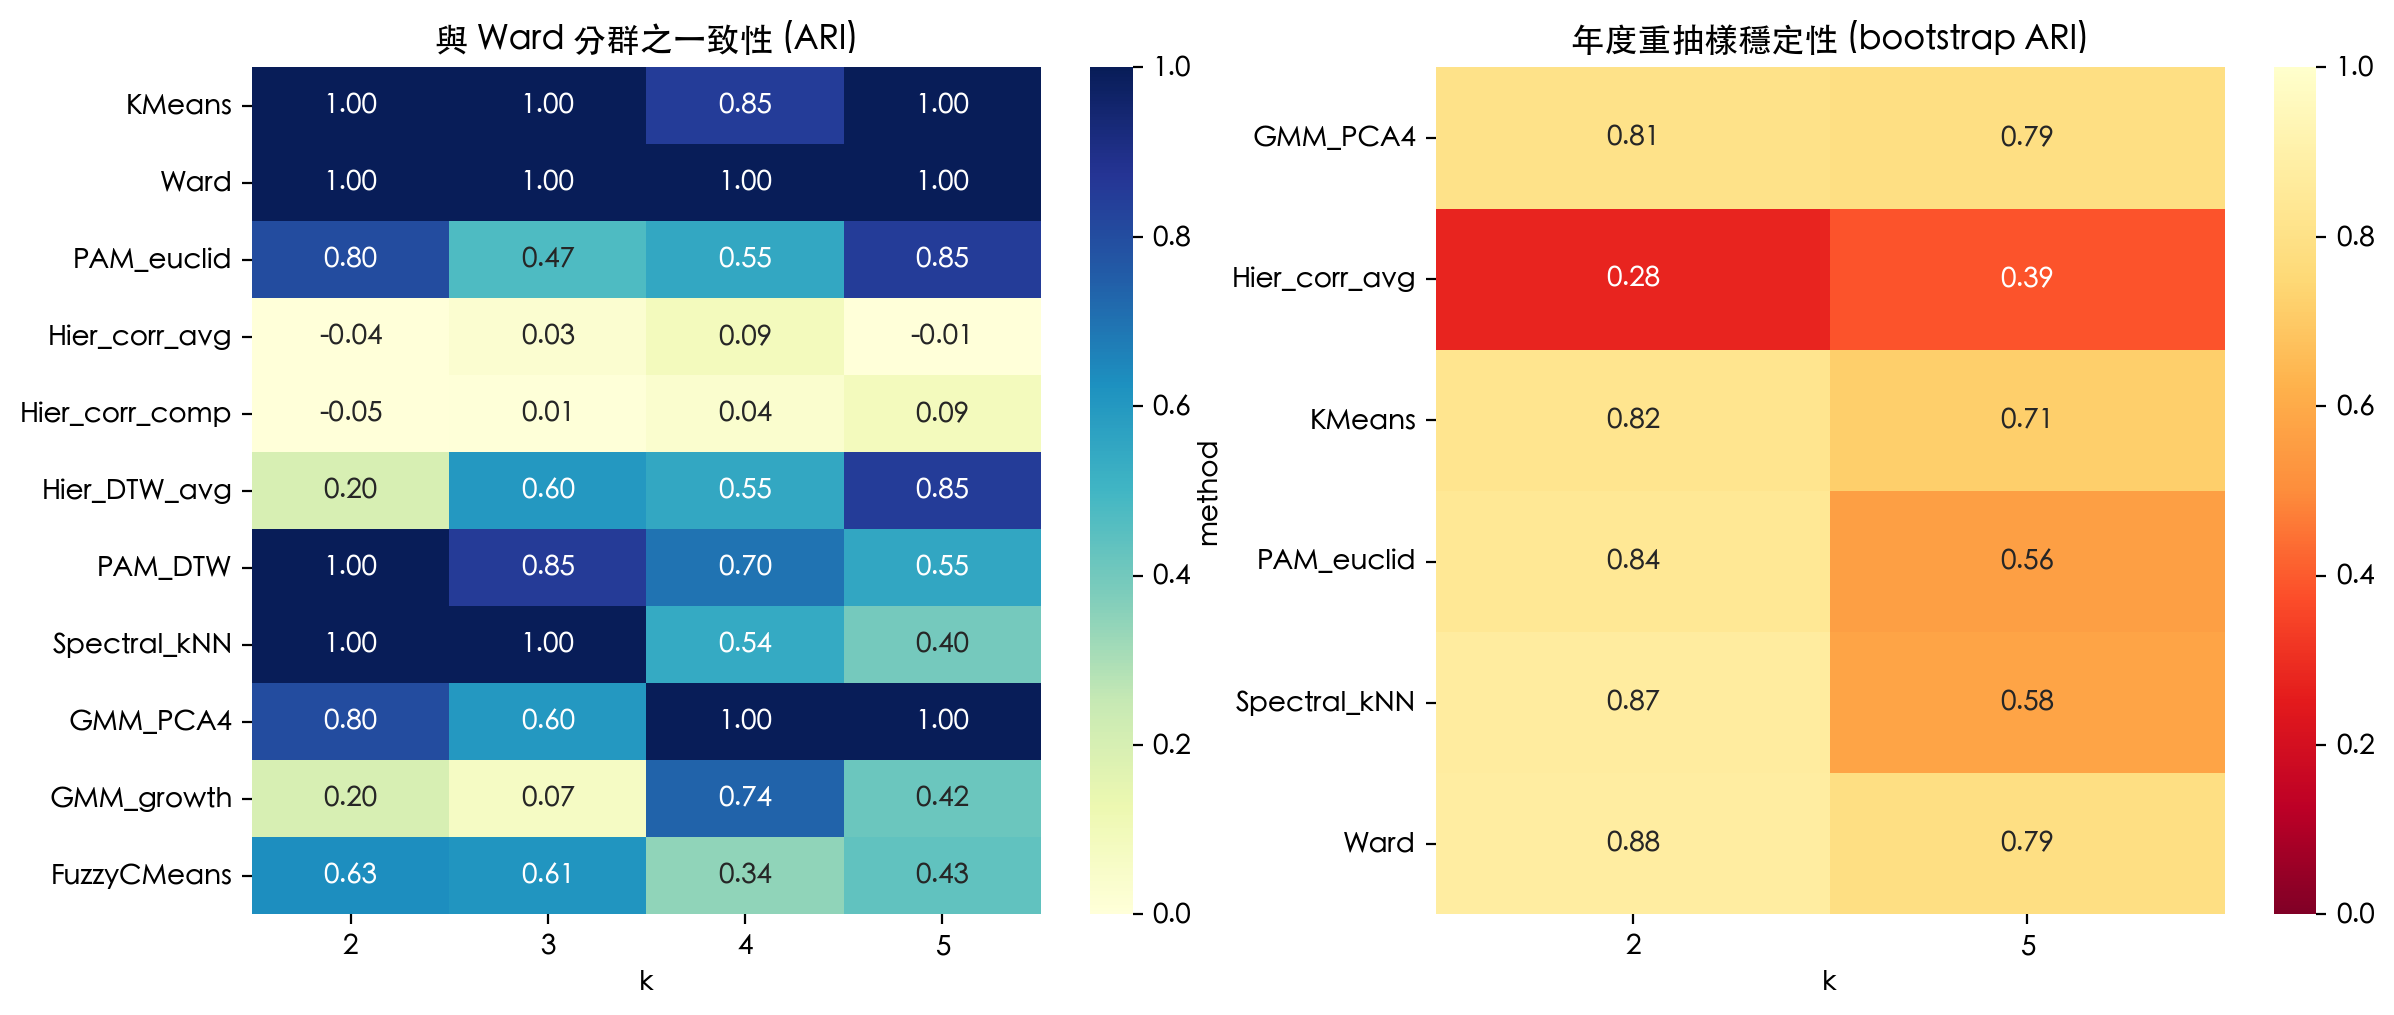
\includegraphics[width=.95\textwidth]{more_cluster_agreement_stability.png}
  \caption{各演算法與Ward分群之一致性（左）與年度重抽樣穩定性（右）。}\label{fig:agree}
\end{figure}

值得注意的是，只看軌跡形狀的分群完全失效。以相關係數距離進行階層式分群時，輪廓係數接近0或為負（不超過0.02），ARI約為0，重抽樣穩定性僅0.28至0.39。這與前述圖像一致：縣市之間的差異在於水準與上升的時點，而不在形狀本身，幾乎所有縣市都呈相似的長期上升型態。以軌跡形狀建立參考群體因此並不適當，分群必須保留水準資訊。模型式與密度式方法則提供了補充訊息：GMM對PCA得分的BIC在 $k=1$ 至5間單調下降（438.7、425.3、343.8、347.7、287.7），於 $k=5$ 最小，但因落在候選範圍邊界，只能說支持「至少5群」；成長曲線係數GMM的BIC在 $k=4$ 最小（125.0），所得分群為南投、屏東、新竹縣、苗栗，台北市，金門縣，以及其餘15縣市，顯示就水準、斜率與曲率而言，台北市（高起點、緩升）與金門（低水準、近年下降）各自獨立。DBSCAN將澎湖與金門標為雜訊，其餘19縣市為同一密集群；模糊C平均（$k=3$）則顯示澎湖縣（最大隸屬度0.40）、花蓮縣（0.43）、新竹市（0.45）與台東縣（0.48）的隸屬度並不集中，較不宜被強制歸入單一群。

綜合而言，北部都會、中西部與南部偏鄉、其餘本島，以及金門與澎湖這個核心結構，被多種獨立的演算法重現，並在重抽樣下相對穩定；宜蘭、嘉義市、新竹市、台南與彰化等邊界縣市的歸屬則隨演算法而異，政策上宜視為過渡區。

\subsection{貝氏階層模型：小區域估計與不確定性}
模型的超參數顯示，全體縣市平均的對數水準、斜率與曲率分別約為3.31、0.39與$-0.11$，縣市間標準差（對數尺度）為0.21、0.14與0.075；過度離散參數 $\phi$ 的後驗平均為2.93（95\%可信區間2.65至3.22），遠大於1，表示只依個案數的Poisson變異會低估年度波動，必須納入額外離散。

部分合併的效果集中於小人口縣市（表\ref{tab:bayes}，圖\ref{fig:forest}）。澎湖縣2018至2022年平均發生率的原始值為52.3，後驗中位數降為46.3（$-11.6\%$），95\%可信區間為40.6至52.4，寬度11.8，為各縣市中最寬；金門縣則由16.9上調至18.3（$+8.4\%$），區間為15.1至21.8。相對地，個案數多的都會區區間很窄（台北市40.0至42.3，新北市40.5至42.5，寬度約2），估計幾乎不受收縮影響。換言之，澎湖原始值之所以居全國之冠，部分來自2019至2020年的高峰（59.4、67.4），收縮與平滑後的估計較保守，但仍在全國最高之列（後驗排名中位數為第1，位居前5名的機率為94\%）。

以後驗樣本計算排名，澎湖縣（前5名機率0.94）、台南市（0.89）、嘉義市（0.79）與彰化縣（0.69）位居前5的機率較高；新北市與台南市高於全體中位數的後驗機率皆為1.00，而南投、苗栗、屏東、花蓮與金門的排名中位數落在第18至21，高於中位數的機率近乎0。嘉義市因人口小而區間較寬（39.3至46.9），宜理解為「可能偏高」而非確定偏高。就趨勢而言，各縣市中期的年增率（後驗中位數）以屏東縣（4.4\%）、澎湖縣（4.1\%）、苗栗縣與台南市（皆約4.0\%）較高，台北市（1.4\%）、基隆市（1.9\%）與金門縣（2.0\%）較低，延續了都會早發緩升、南部與偏鄉追趕的圖像，並補上了可信區間。

\begin{table}[H]
\centering
\caption{貝氏階層模型之2018--2022年平均發生率估計（每10萬人口；依後驗中位數由高至低；僅列代表性縣市，完整表見\texttt{bayes\_county\_summary.csv}）。}\label{tab:bayes}
\small
\begin{tabular}{lrrrrr}
\toprule
縣市 & 原始 & 後驗中位數 & 95\%可信區間 & 排名中位數 & 前5名機率\\
\midrule
澎湖縣 & 52.3 & 46.3 & 40.6--52.4 & 1 & 0.94\\
嘉義市 & 44.1 & 43.2 & 39.3--46.9 & 2 & 0.79\\
台南市 & 44.6 & 42.5 & 41.3--44.0 & 3 & 0.89\\
彰化縣 & 42.9 & 42.1 & 40.4--43.8 & 4 & 0.69\\
新北市 & 42.0 & 41.5 & 40.5--42.5 & 6 & 0.38\\
台北市 & 41.5 & 41.1 & 40.0--42.3 & 8 & 0.16\\
屏東縣 & 35.4 & 34.9 & 33.1--36.8 & 18 & 0.00\\
苗栗縣 & 35.7 & 34.5 & 32.3--36.8 & 18 & 0.00\\
南投縣 & 35.2 & 34.1 & 31.8--36.3 & 19 & 0.00\\
金門縣 & 16.9 & 18.3 & 15.1--21.8 & 21 & 0.00\\
\bottomrule
\end{tabular}
\end{table}

\begin{figure}[H]
  \centering
  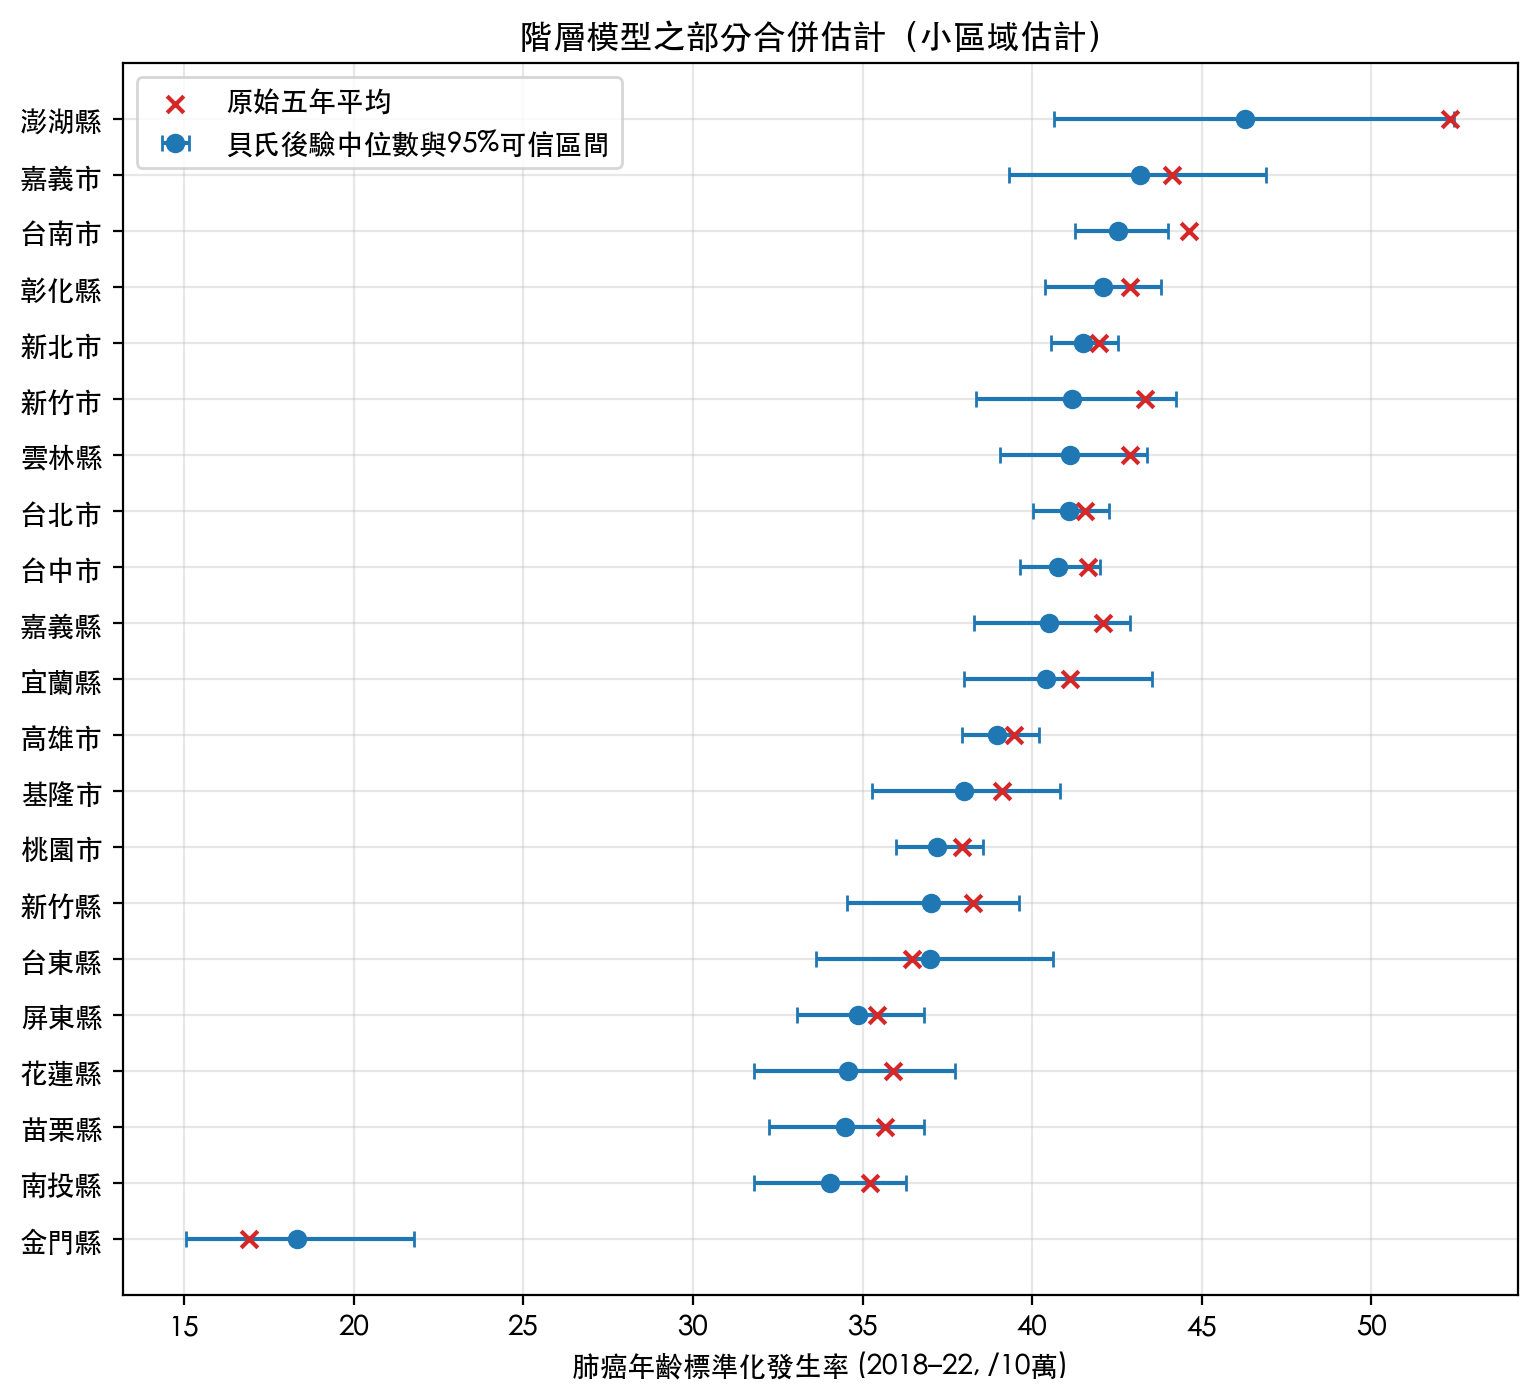
\includegraphics[width=.78\textwidth]{bayes_forest_2018_22.png}
  \caption{原始五年平均（紅叉）與貝氏後驗中位數及95\%可信區間（藍點）。}\label{fig:forest}
\end{figure}

\begin{figure}[H]
  \centering
  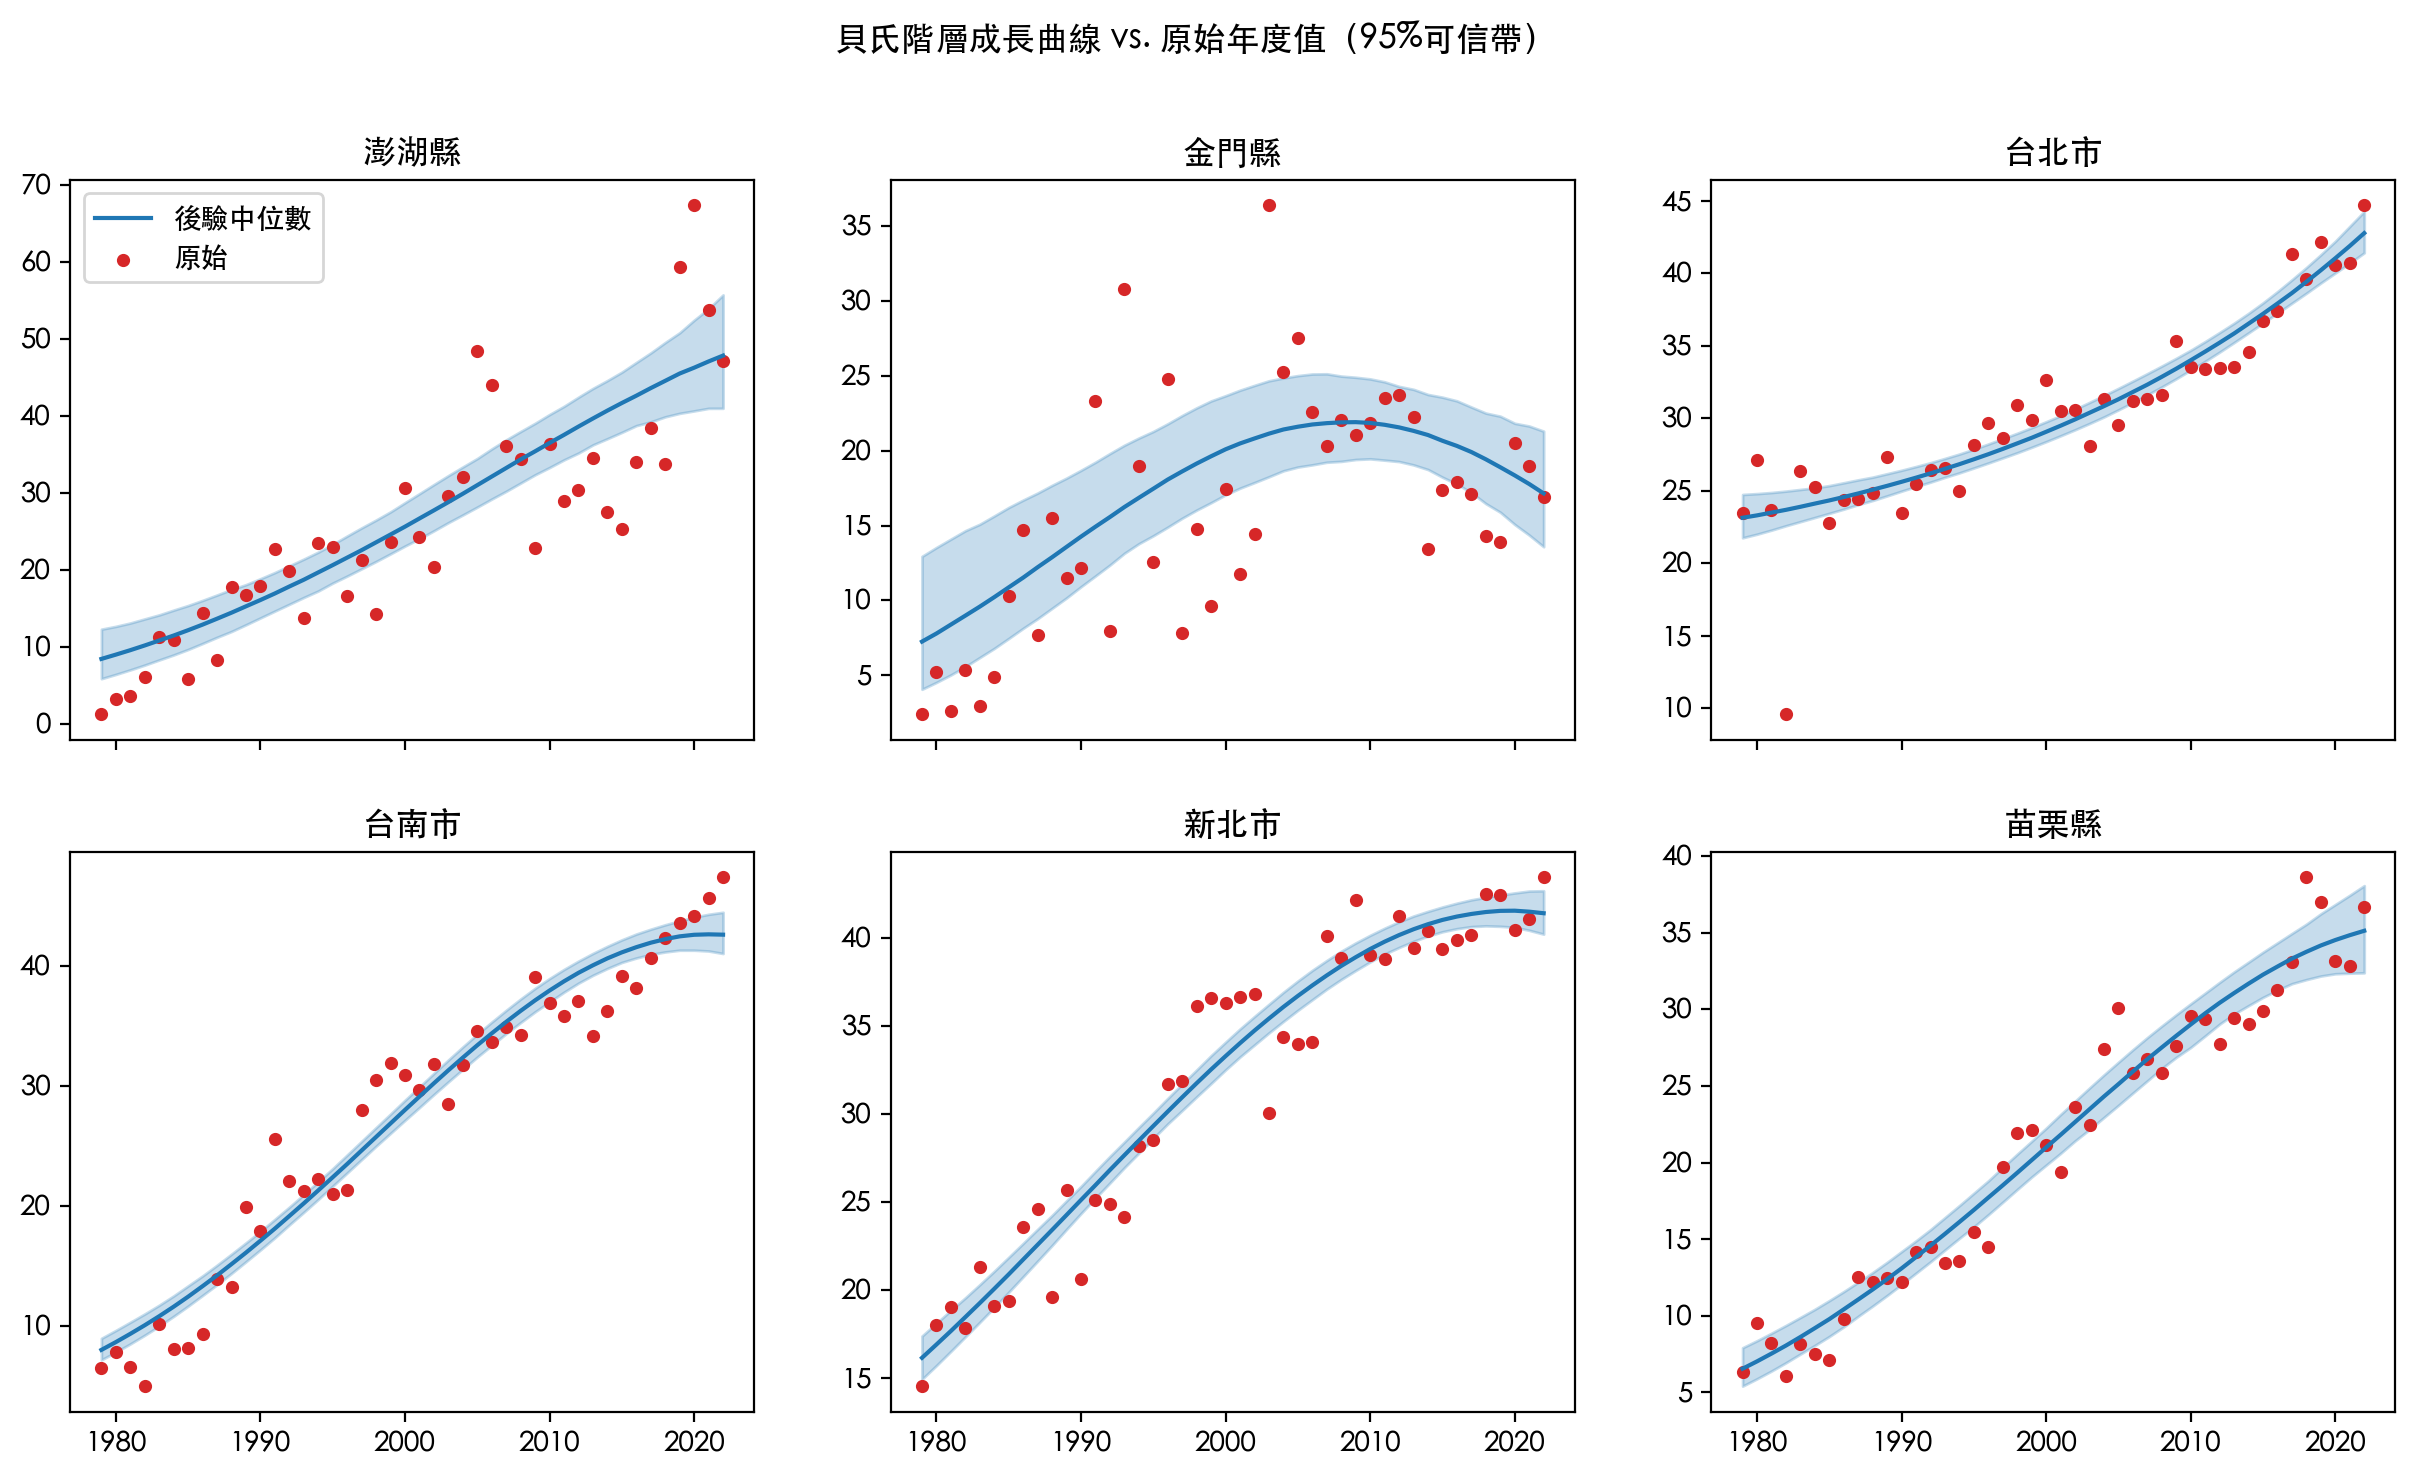
\includegraphics[width=\textwidth]{bayes_trajectories.png}
  \caption{代表性縣市之貝氏階層成長曲線與原始年度值。二次曲線平滑了小人口縣市的波動，但在末端（如台北市2022年、澎湖2019至2020年的高點）會有低估。}\label{fig:traj}
\end{figure}

把不確定性帶進分群後（對後驗樣本分群所得的同群機率），金門縣與澎湖縣各自獨立（機率1.00）；北部都會群（台北、新北、基隆）內部的最低配對機率為0.33，因為台北市（高起點、曲率大）與新北、基隆的曲線形狀不同；中西部南部偏鄉群內部最低為0.74；而佔12個縣市的「其餘本島」群內部最低配對機率僅0.03，代表該群內部異質性大，分群結果對這一群最不穩。

\subsection{空間自相關與空間約束分群}
1979至1983年的發生率具有顯著的正空間自相關（Moran's $I=0.53$，置換檢定 $p=0.001$），也就是發生率高的縣市彼此相鄰（以北部都會為主）。然而2018至2022年的 $I=-0.24$（$p=0.92$），已無正自相關，逐年平均的 $I$ 也由1979至1989年的0.31降至2010至2022年的$-0.01$（圖\ref{fig:moran}）。PC1得分（長期穩定的梯度）仍有微弱的空間自相關（$I=0.25$，$p=0.036$），1979至2022年的增幅則沒有（$I=-0.02$，$p=0.43$；PC2得分 $I=0.04$，$p=0.27$）。縣市間發生率的空間群聚因此已經消失，與前述變異係數由0.61降至0.16的收斂一致。從公共衛生的角度看，早期高風險集中在相連的都會區，適合以區域為單位部署資源；如今風險已經擴散，高低發生率的縣市在地理上交錯分布，區域性的粗略策略效益下降，宜改以縣市甚至鄉鎮層級的目標性介入。

\begin{figure}[H]
  \centering
  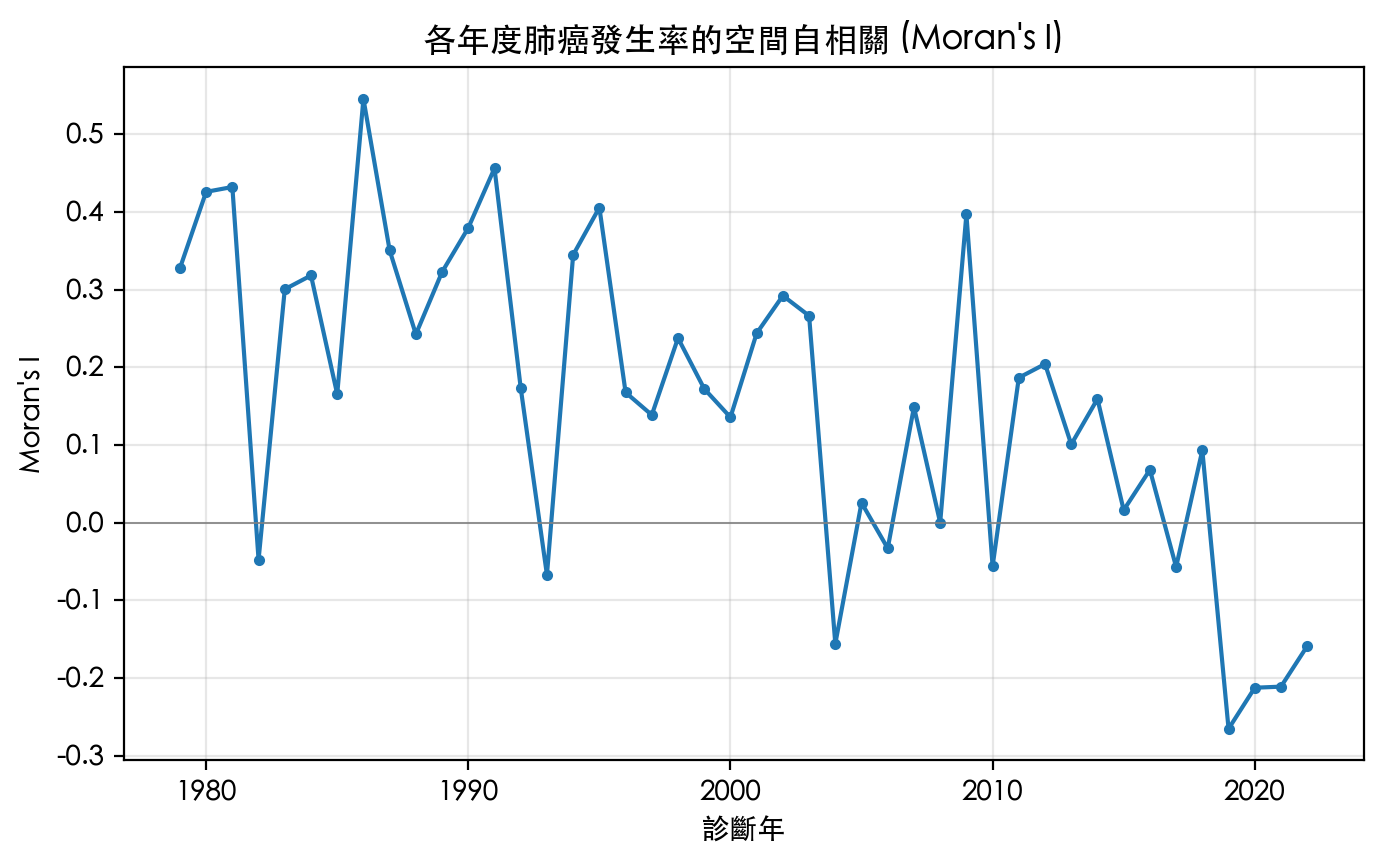
\includegraphics[width=.62\textwidth]{moran_i_by_year.png}
  \caption{各年度肺癌發生率的Moran's $I$：1980年代為正（空間群聚），2010年後接近0或為負。}\label{fig:moran}
\end{figure}

空間約束下，群內縣市必然地理相連。$k=5$的分群為：北部都會（台北、新北、基隆），新竹市、新竹縣與苗栗縣，東南部（南投、台東、屏東、花蓮），金門縣，以及其餘西部與宜蘭、桃園、澎湖共10個縣市（表\ref{tab:spatial}，圖\ref{fig:spmap}）。與無約束的Ward（$k=5$）相比，北部都會群與金門縣不變，但無約束分群中的「中西部南部偏鄉群」（南投、屏東、新竹縣、苗栗）在空間約束下被拆為地理上不相連的兩部分：新竹縣與苗栗縣併入新竹市，南投與屏東則與台東、花蓮併為東南部群；澎湖縣在 $k=5$ 時因鄰接設定而併入西部大群，要到 $k=6$ 才單獨成群。兩種觀點並不矛盾：就發生率軌跡而言，南投、屏東與新竹縣、苗栗相似；就地理連續性而言，它們分屬東南部與北中部兩片區域。

\begin{table}[H]
\centering
\caption{空間約束Ward（$k=5$）之分群及群內縣市平均之發生率（每10萬人口）。}\label{tab:spatial}
\small
\begin{tabular}{l p{7.6cm} cc}
\toprule
群 & 成員 & 1979--83 & 2018--22\\
\midrule
北部都會 & 台北市、基隆市、新北市 & 19.0 & 40.9\\
西部與宜蘭、桃園、澎湖 & 台中市、台南市、嘉義市、嘉義縣、宜蘭縣、彰化縣、桃園市、澎湖縣、雲林縣、高雄市 & 10.1 & 42.9\\
新竹—苗栗 & 新竹市、新竹縣、苗栗縣 & 9.0 & 39.1\\
東南部 & 南投縣、台東縣、屏東縣、花蓮縣 & 8.5 & 35.8\\
金門 & 金門縣 & 3.7 & 16.9\\
\bottomrule
\end{tabular}
\end{table}

\begin{figure}[H]
  \centering
  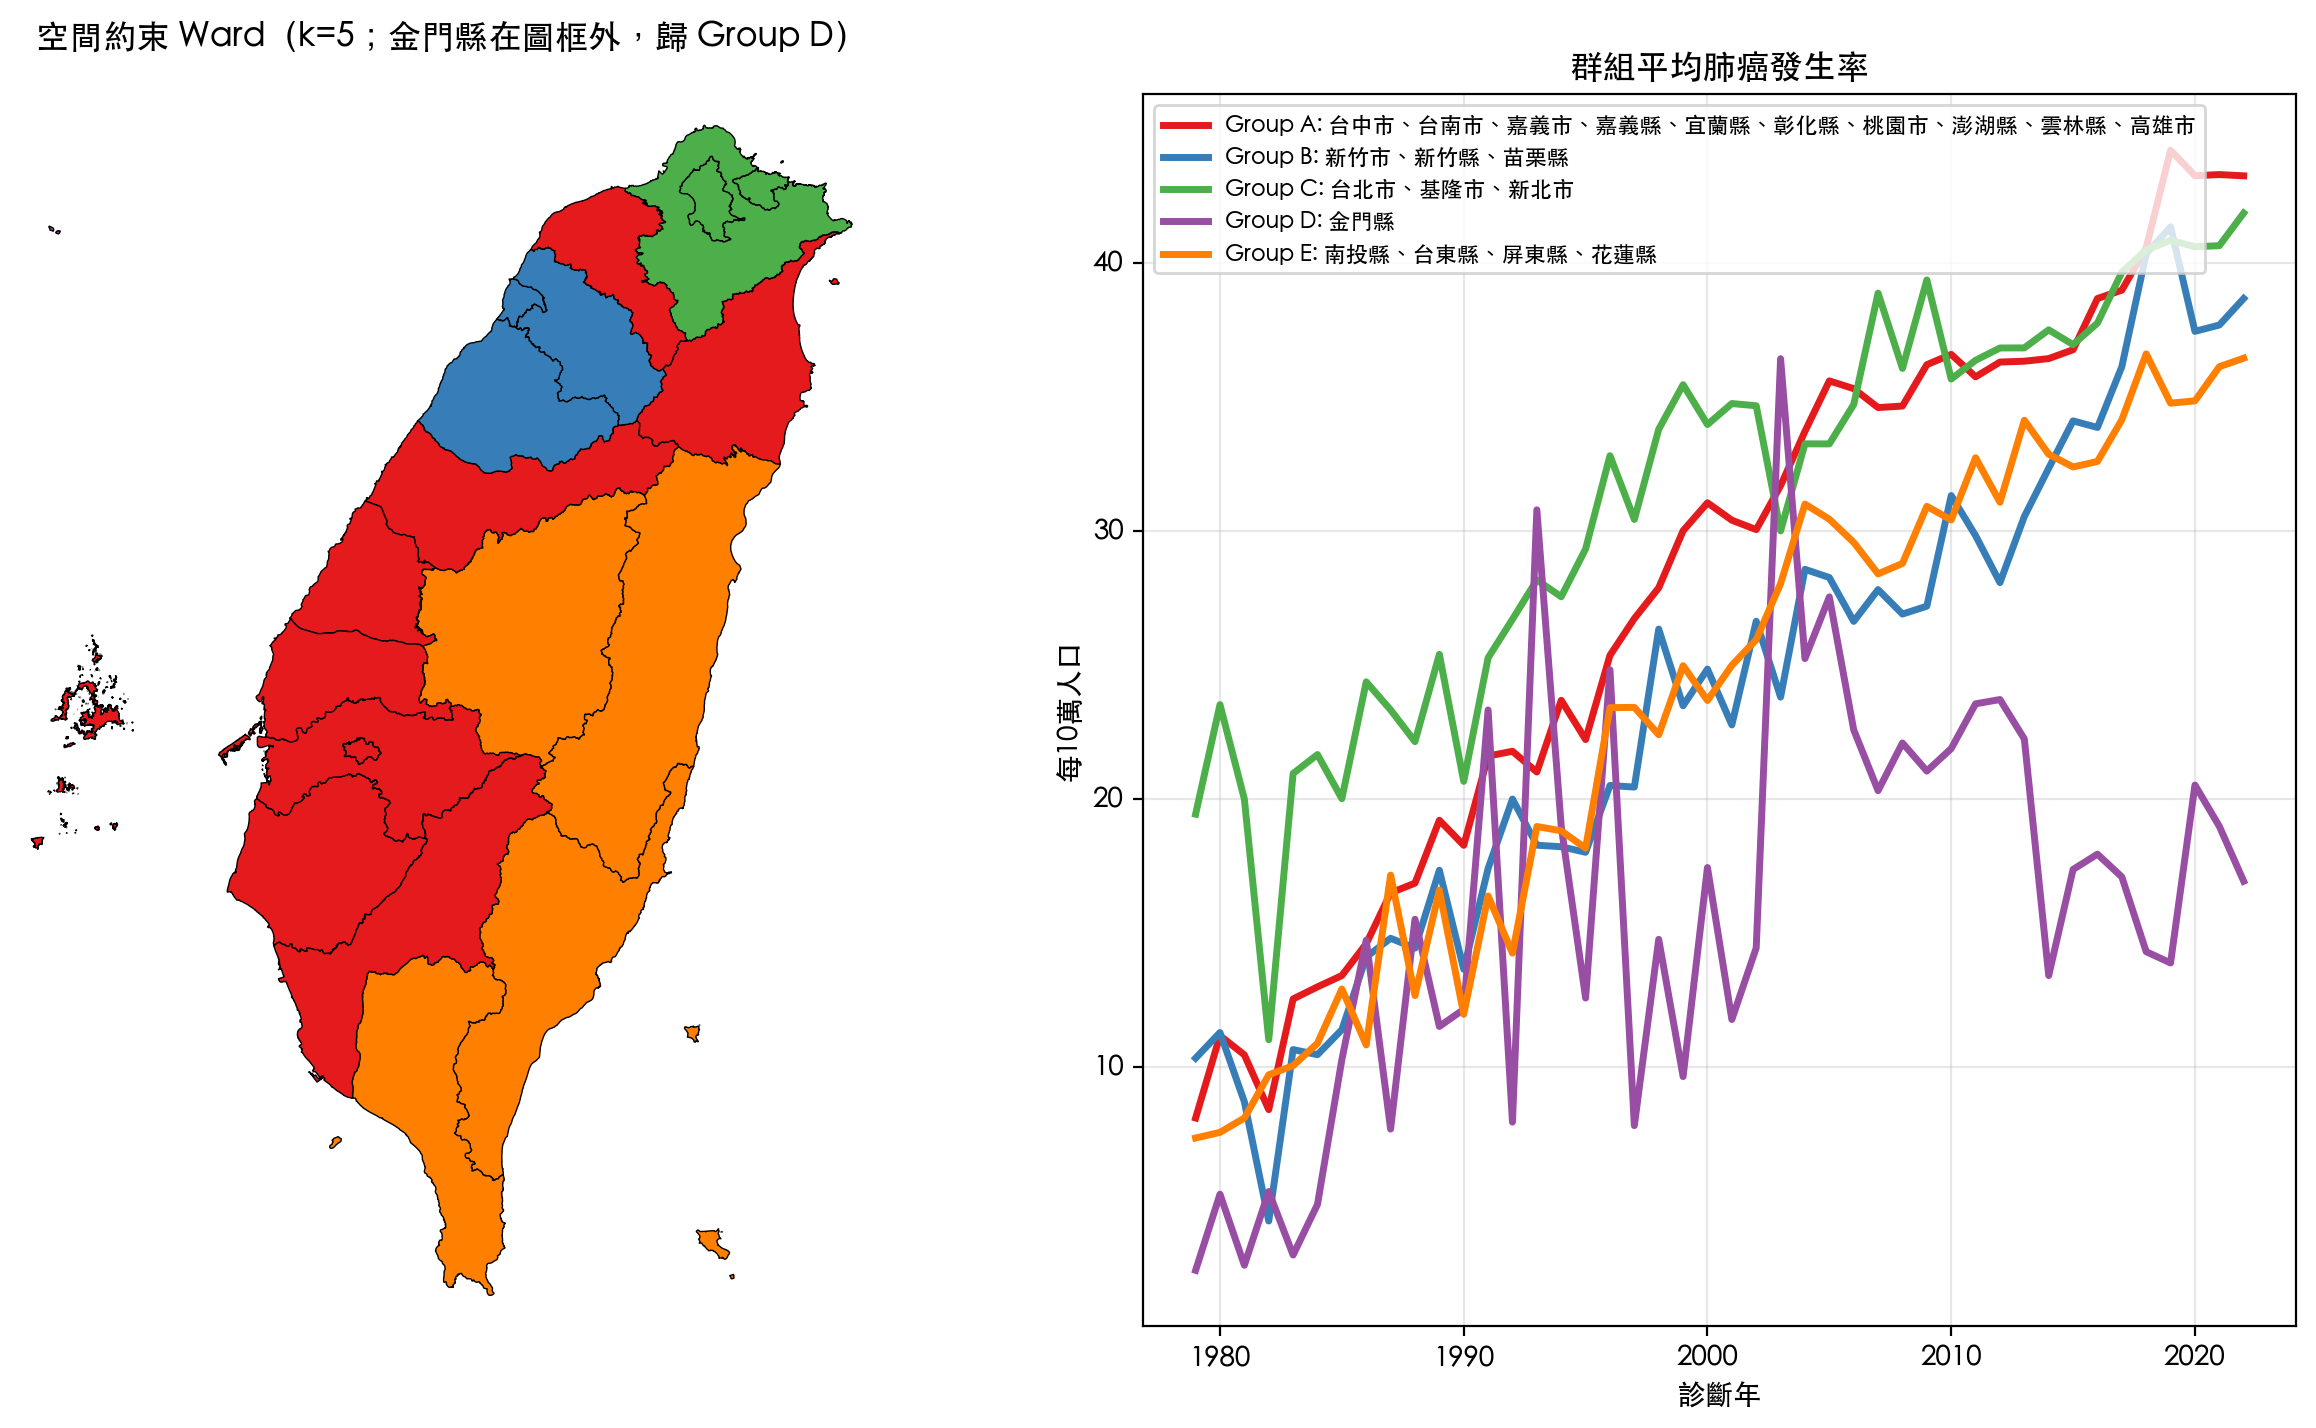
\includegraphics[width=\textwidth]{spatial_ward_map_k5.png}
  \caption{空間約束Ward（$k=5$）之地圖（左；金門縣在圖框外）與各群平均軌跡（右）。}\label{fig:spmap}
\end{figure}

空間約束的代價是群內同質性下降。輪廓係數在 $k=5$ 為0.093（無約束為0.252），$k=4$ 為0.086（0.235），$k=3$ 為0.206（0.244），與無約束分群的ARI僅0.37至0.49；無約束分群在 $k=5$ 時其實由8塊互不相連的地理片段組成（$k=2$為6塊、$k=3$為7塊、$k=6$為12塊），可見軌跡相似性與地理鄰近性是不同的概念。$k=2$時空間約束分群的輪廓係數（0.461）反而較高，但同樣只是把金門縣孤立（ARI 0.20）。因此，若分群的目的是建立參考母體以借力估計，應採用無約束分群或貝氏階層模型；若目的是劃分行政或資源配置的區域，則採用空間約束分群，並接受群內同質性較低。

\subsection{發生與死亡：兩端指標的落差}
全國21縣市平均的ASMR在2020至2025年間約為21.6至22.9（男性約30至32，女性約15），男性約為女性的兩倍。各縣市2020至2022年三年平均的ASIR、ASMR、MIR及分性別ASMR列於附錄表\ref{tab:mir}。發生率與死亡率在縣市間的相關係數僅為0.53（2020年）、0.34（2021年）與0.33（2022年），意味著只依其中一個指標配置資源，可能遺漏另一端的重點地區（圖\ref{fig:scatter}）。

台北市的發生率偏高（42.0），但死亡率為全國最低（17.4），MIR僅0.42，為本島最低，與都會區較佳的醫療可近性、較便利的篩檢與就診，以及較早期的診斷相符，不過也可能受癌別組織型與人口社經特徵影響，本研究無法拆解。相反地，屏東、台東與花蓮的發生率並不高（35至37，低於全國平均），死亡率卻偏高（23.7至24.3），MIR約0.66至0.69，這是值得公共衛生系統關注的訊號：在偏遠或醫療資源較薄弱的地區，可能存在較晚期診斷、轉診與治療可近性不足的問題。雲林縣與嘉義縣的發生率與死亡率都在全國前段（死亡率27.6與27.1），男性ASMR（38.9與39.6）為全國最高，顯示男性肺癌負擔沉重，宜併同吸菸盛行、職業暴露及地區環境因素檢視。澎湖縣的發生率最高（56.2），但死亡率僅居中高（25.2，MIR 0.46），且女性ASMR（20.5）為全國最高，不過澎湖每年肺癌死亡僅約50至60例，估計不穩。金門縣的發生率（18.8）與死亡率（17.8）幾乎相等，MIR高達0.95，幾乎不可能是真實的存活情形，較可能是登記面的落差，例如居民至本島就醫的診斷個案被計入其他縣市，或發生率被低估，而死亡依登記地歸屬，此點宜以個案層級的居住地與就醫地資料驗證。\note{金門之解釋為合理推測，需查證}

\begin{figure}[H]
  \centering
  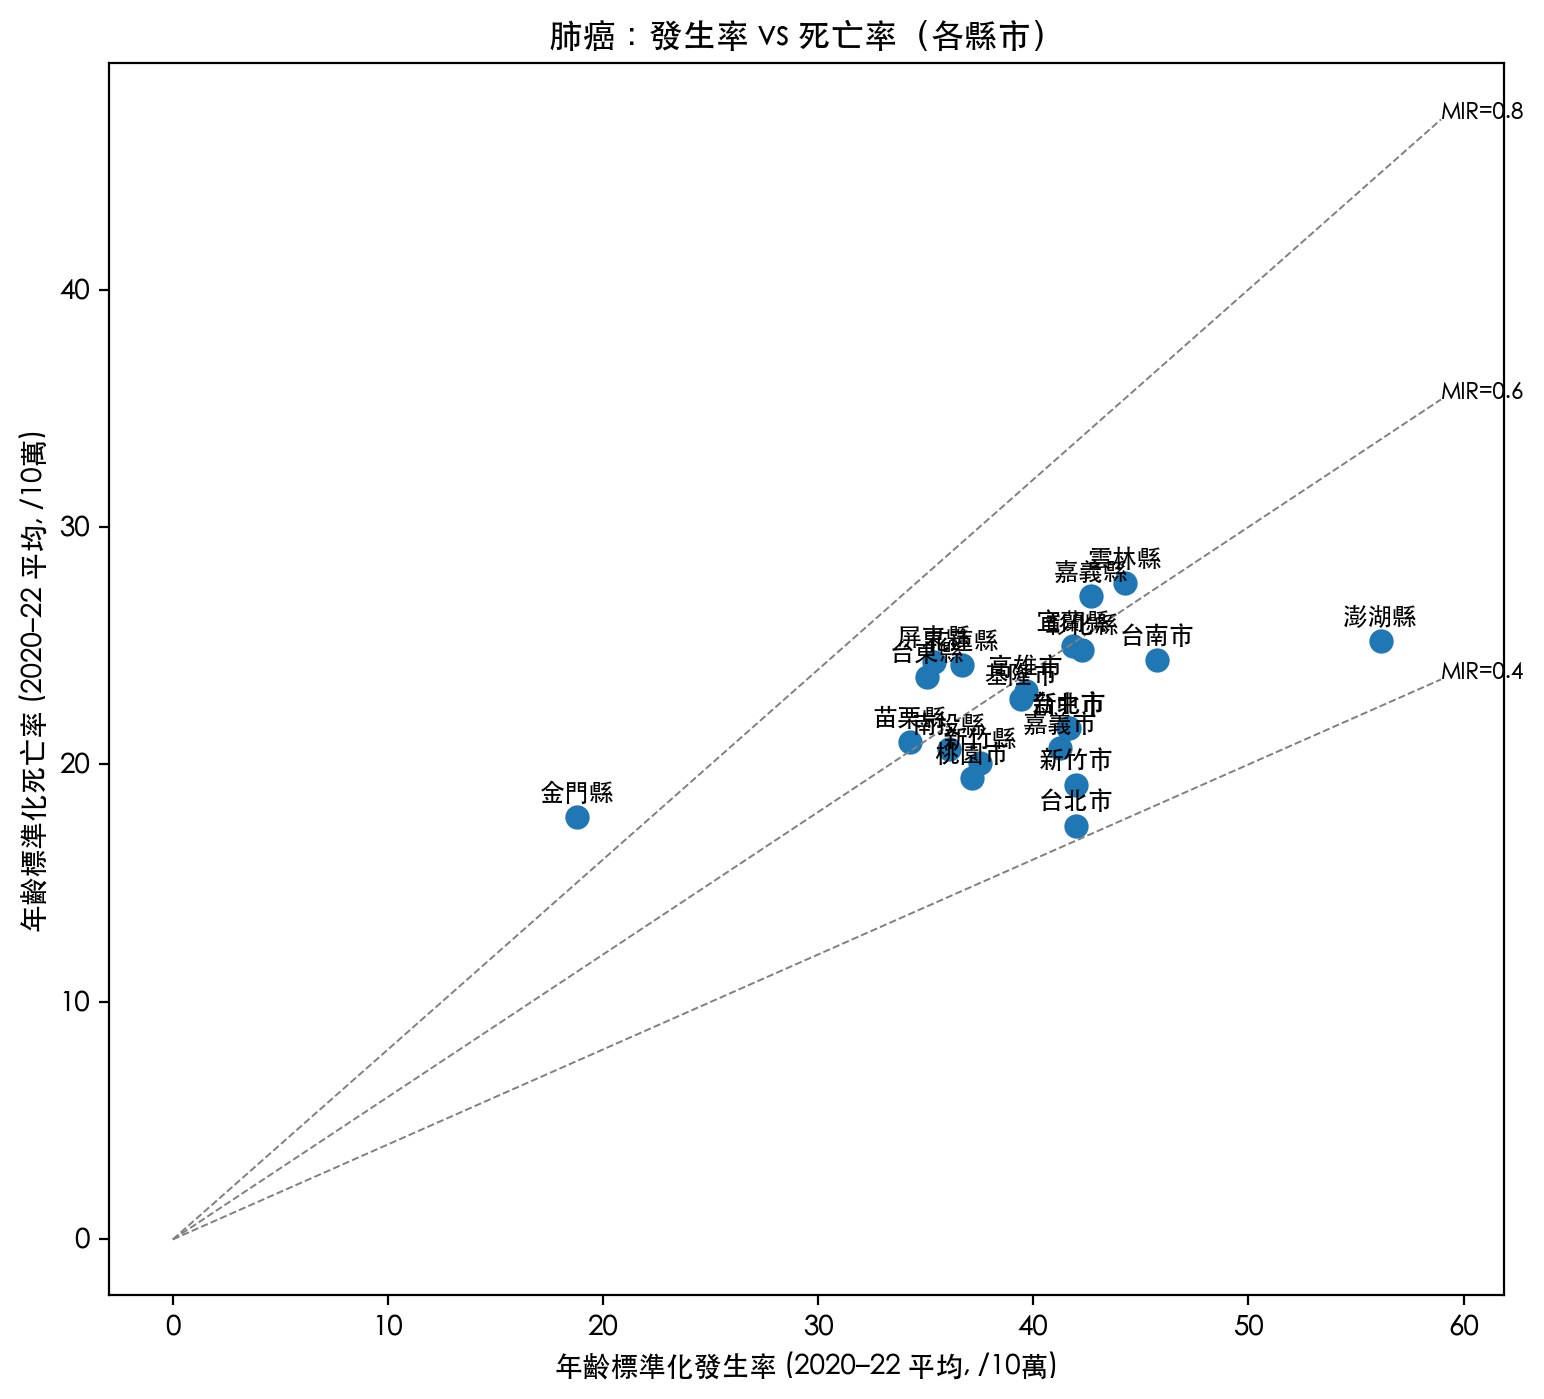
\includegraphics[width=.72\textwidth]{incidence_vs_mortality_scatter.png}
  \caption{各縣市肺癌發生率與死亡率（2020--2022年平均）；虛線為MIR等值線。}\label{fig:scatter}
\end{figure}

%=====================================================================
\section{討論}
%=====================================================================
本研究描繪的是一個「整體墊高、差距收斂、空間群聚消失」的過程，而肺癌的長潛伏期是理解它的關鍵。今日的發生率反映的是二、三十年前的吸菸與環境暴露，1979至2022年發生率的持續攀升，與台灣在1970至1990年代男性吸菸盛行較高、其後人口老化使高風險族群累積的圖像一致\note{可補充國民健康署成人吸菸行為調查之歷年吸菸率並標示出處}。年齡標準化雖已校正年齡結構，卻不能排除世代效應，也就是不同出生世代的吸菸史；年齡—時期—世代模型將是回答「政策是否見效」更直接的方法。同理，2009年之後菸害防制的強化與2023年電子煙及加熱菸的納管，其效益可能要待後續年度才可見。

PC1呈現的穩定梯度提醒我們，肺癌風險的地區差異並非短期現象。從公共衛生角度，可能的解釋包括個人行為（如吸菸與嚼檳榔等複合暴露的地區分布）、職業與環境暴露（空氣污染、烹飪油煙）、社會經濟與教育程度，以及醫療可近性與診斷能力。中南部空氣品質較差是常被提出的環境假說，但本研究僅以縣市層級的標準化率作描述，無法作因果推論；要檢驗它，需要加入縣市或更細的鄉鎮層級的暴露指標與吸菸率，並使用空間迴歸或多層次模型。Moran's $I$的結果則顯示，早期集中於相連都會區的風險如今已擴散，區域性的粗略策略已不如針對縣市與鄉鎮的目標性介入適用；也因為所有結論都建立在縣市層級的資料上，必須避免生態學謬誤（Robinson, 1950），亦即不能因為某縣市發生率較高，就推論該縣市每個人或特定族群的風險較高，目標人群的選擇仍需要個案層級或更細緻分層的資料。

在死亡率資料中，女性ASMR約為男性的一半，但各縣市的女性值並不低（澎湖20.5、雲林18.1、台南17.0）。台灣女性肺癌以肺腺癌為主，且相當比例發生在不吸菸者，與二手菸、烹飪油煙、空氣污染及家族史等相關，因此公共衛生策略不宜只針對吸菸者，也應涵蓋室內空氣與家戶炊事暴露的衛教與改善，以及對具家族史的非吸菸者的風險評估。本資料僅提供全性別發生率，未來宜分性別、分組織型（腺癌、鱗狀細胞癌、小細胞癌）重複相同的分析。

發生與死亡兩端指標的落差，則與早期偵測及醫療可近性直接相關。國民健康署自2022年7月起推動肺癌早期偵測計畫，以低劑量電腦斷層（LDCT）針對重度吸菸者與具肺癌家族史者提供篩檢\note{請核對方案起訖與對象條件}。由於這項計畫的實施只涵蓋本分析的末期，2020至2022年的MIR主要反映篩檢普及之前的情況，可作為政策實施的基線。MIR的縣市差異（台北0.42，屏東與台東0.69）提示偏鄉與東部縣市可能面對較晚期診斷與治療可近性不足的問題；而當LDCT篩檢擴大時，發生率會因篩檢而短期上升（先導時間與過度診斷），MIR則應下降，所以評估篩檢成效時應同時監測發生率、期別分布與死亡率，不能只因發生率上升就判定情勢惡化。

最後，小人口縣市的估計問題與參考母體的概念值得合併討論。貝氏階層模型與分群都是借力的做法：前者以模型向全體平均收縮並量化不確定性，後者將軌跡相似的縣市歸併為參考群體，在群內估計較穩定的基準發生率與趨勢。分群的結果顯示，北部都會群、其餘本島與中西部南部偏鄉群可作為資源配置與目標設定的三個主要單位，而澎湖與金門需要以較長的移動平均或貝氏平滑估計後再解讀。這些結論也與演算法選擇有關：K-means、Ward與GMM重現了同一個核心結構，邊界縣市則依方法而異，故宜視為過渡區；只看軌跡形狀的分群無效，說明水準資訊是分群的核心；若目的在於劃分行政區域，則需要空間約束分群，並接受群內同質性較低的代價。

%=====================================================================
\section{政策與實務建議}
%=====================================================================
首先，考量肺癌的長潛伏期，菸害防制應被視為長期投資，建議以世代吸菸率與初次吸菸年齡作為過程指標，並將電子煙與加熱菸納入監測。其次，發生率與死亡率的縣市排序相關僅0.33至0.53，資源配置不宜只依其中一個指標；MIR偏高的縣市（屏東、台東、花蓮、嘉義縣、雲林縣等）宜優先檢視篩檢可近性、轉診與治療網絡。第三，LDCT篩檢擴大後，應以本研究2020至2022年的縣市別基線為對照，同時追蹤發生率、期別與MIR的聯合變化，避免對篩檢成效作出誤判。第四，非吸菸者與女性的風險需要被納入，包括家族史與環境暴露的風險評估，以及室內空氣與炊事暴露的衛教與改善。第五，對離島與小人口縣市，應以多年合併、參考群體或貝氏平滑估計率值，並在公布時附上個案數與信賴區間。最後，應改善個案層級居住地與就醫地的串聯，以降低登記地歸屬造成的偏差，金門縣的異常MIR便是一例。

%=====================================================================
\section{研究限制與未來工作}\label{sec:limit}
%=====================================================================
本研究有幾項限制需要說明。首先，死亡資料的時間窗口很短：目前只取得2020至2023年與2025年的縣市別死亡率，1979至2022年的完整死亡率序列需另自衛生福利部歷年死因統計取得，取得之後本專案的PCA與分群流程可直接套用並與發生率對照。其次，1979年起的癌症登記在早年各地的完整性可能不一，使早期縣市間的差異（變異係數0.61）部分來自測量而非真實風險；金門、澎湖（及早年之連江）個案數少，標準化率不穩定，其獨立成群與PC3、PC4的極端得分應謹慎解讀。第三，MIR是同年標準化率相除，未考慮診斷至死亡的時間落差、篩檢造成的過度診斷，以及居住地與就醫地不同造成的歸屬偏差，2020至2022年也受COVID-19疫情影響醫療利用。第四，PCA與分群使用的欄標準化移除了全國的年度水準，它描述的是相對結構，若關心全國趨勢，須搭配第\ref{sec:trend}節的描述統計。第五，輪廓係數整體偏低（最高0.35至0.46，且 $k=2$ 的高值可由金門孤立解釋），表示縣市之間沒有截然分離的群聚，分群應視為方便的歸納而非天然分類。第六，貝氏階層模型採二次曲線，對末端與突發高峰會有低估，也沒有納入空間先驗或年齡—時期—世代效應；空間約束分群的結果則取決於離島鄰接關係的人為設定。最後，本文未納入吸菸率、空氣污染、社經指標與醫療資源等共變量，後續可以空間迴歸、年齡—時期—世代模型與帶有空間先驗的貝氏小區域模型加以擴充。

%=====================================================================
\section*{參考文獻}
%=====================================================================
\begin{small}
\begin{thebibliography}{99}
  \bibitem{r1} Ahmad OB, Boschi-Pinto C, Lopez AD, Murray CJL, Lozano R, Inoue M. \emph{Age standardization of rates: a new WHO standard}. GPE Discussion Paper Series No.\ 31. World Health Organization; 2001.
  \bibitem{r2} Jolliffe IT. \emph{Principal Component Analysis}, 2nd ed. New York: Springer; 2002.
  \bibitem{r3} Lloyd SP. Least squares quantization in PCM. \emph{IEEE Trans Inf Theory}. 1982;28(2):129--137.
  \bibitem{r4} Rousseeuw PJ. Silhouettes: a graphical aid to the interpretation and validation of cluster analysis. \emph{J Comput Appl Math}. 1987;20:53--65.
  \bibitem{r5} Robinson WS. Ecological correlations and the behavior of individuals. \emph{Am Sociol Rev}. 1950;15(3):351--357.
  \bibitem{r6} Ward JH. Hierarchical grouping to optimize an objective function. \emph{J Am Stat Assoc}. 1963;58(301):236--244.
  \bibitem{r7} 衛生福利部國民健康署。癌症登記資料（肺癌發生率，1979--2022）。\note{請補正式資料集名稱與取得日期}
  \bibitem{r8} 衛生福利部統計處。死因統計結果分析與各縣市統計表（民國109--112、114年）。
  \bibitem{r9} 內政部國土測繪中心。直轄市、縣（市）界線（1140318版）。
  \bibitem{r10} 陳玟儒（2024）。臺灣居民的全死因及主要死因時空分析。\note{請補齊出處（學位論文／期刊）}
  \bibitem{r11} 楊敬賢等（2014）；江信緯（2015）；de Simone E, et al.\ (2012)。\note{請補齊書目格式}
\end{thebibliography}
\end{small}

%=====================================================================
\appendix
\section{附表}
%=====================================================================
\begin{table}[H]
\centering
\caption{各縣市發生率變化、PCA得分與分群（$k=5$）。發生率為五年平均（每10萬人口）；PC1、PC2為相關係數矩陣PCA之縣市得分；群代號對應表\ref{tab:clusters}：A為其餘本島，B為金門，C為中西部與南部偏鄉，D為北部都會，E為澎湖。}\label{tab:counties}
\small
\begin{tabular}{lrrrrrc}
\toprule
縣市 & 1979--83 & 2018--22 & 倍數 & PC1 & PC2 & 群\\
\midrule
金門縣 & 3.7 & 16.9 & 4.6 & $-13.16$ & $5.35$ & B\\
南投縣 & 7.6 & 35.2 & 4.6 & $-5.32$ & $-0.23$ & C\\
屏東縣 & 6.2 & 35.4 & 5.7 & $-6.07$ & $-1.50$ & C\\
苗栗縣 & 7.7 & 35.7 & 4.6 & $-6.50$ & $-1.13$ & C\\
花蓮縣 & 10.3 & 35.9 & 3.5 & $-1.49$ & $1.36$ & A\\
台東縣 & 10.0 & 36.5 & 3.7 & $-0.88$ & $-0.64$ & A\\
桃園市 & 12.9 & 37.9 & 3.0 & $1.85$ & $0.81$ & A\\
新竹縣 & 8.2 & 38.3 & 4.7 & $-5.05$ & $-0.03$ & C\\
基隆市 & 16.7 & 39.1 & 2.3 & $6.31$ & $3.43$ & D\\
高雄市 & 10.0 & 39.5 & 3.9 & $-0.05$ & $-0.69$ & A\\
宜蘭縣 & 10.4 & 41.1 & 3.9 & $4.86$ & $-0.88$ & A\\
台北市 & 22.0 & 41.5 & 1.9 & $5.19$ & $4.71$ & D\\
台中市 & 13.0 & 41.6 & 3.2 & $1.70$ & $-0.44$ & A\\
新北市 & 18.1 & 42.0 & 2.3 & $7.22$ & $1.75$ & D\\
嘉義縣 & 10.5 & 42.1 & 4.0 & $3.24$ & $-0.74$ & A\\
雲林縣 & 9.0 & 42.9 & 4.8 & $1.00$ & $-2.01$ & A\\
彰化縣 & 10.0 & 42.9 & 4.3 & $3.04$ & $-2.10$ & A\\
新竹市 & 11.2 & 43.3 & 3.9 & $1.17$ & $0.77$ & A\\
嘉義市 & 13.2 & 44.1 & 3.3 & $3.34$ & $0.90$ & A\\
台南市 & 7.2 & 44.6 & 6.2 & $1.20$ & $-2.96$ & A\\
澎湖縣 & 5.1 & 52.3 & 10.3 & $-1.60$ & $-5.73$ & E\\
\bottomrule
\end{tabular}
\end{table}

\begin{table}[H]
\centering
\caption{各縣市肺癌ASIR、ASMR、MIR與分性別ASMR（2020--2022年平均；每10萬人口；依MIR排序）。}\label{tab:mir}
\small
\begin{tabular}{lrrrrr}
\toprule
縣市 & ASIR & ASMR & MIR & 男ASMR & 女ASMR\\
\midrule
台北市 & 42.0 & 17.4 & 0.42 & 22.9 & 13.1\\
澎湖縣 & 56.2 & 25.2 & 0.46 & 32.9 & 20.5\\
新竹市 & 42.0 & 19.2 & 0.46 & 26.5 & 13.4\\
新北市 & 41.7 & 21.5 & 0.52 & 29.6 & 14.9\\
台中市 & 41.6 & 21.6 & 0.52 & 29.6 & 14.8\\
嘉義市 & 41.3 & 20.7 & 0.52 & 30.9 & 12.8\\
桃園市 & 37.1 & 19.4 & 0.52 & 26.4 & 13.4\\
台南市 & 45.8 & 24.4 & 0.53 & 32.9 & 17.0\\
新竹縣 & 37.5 & 20.1 & 0.53 & 26.9 & 13.8\\
南投縣 & 36.1 & 20.6 & 0.57 & 28.8 & 13.1\\
基隆市 & 39.4 & 22.8 & 0.58 & 29.9 & 16.8\\
高雄市 & 39.7 & 23.1 & 0.58 & 31.7 & 15.8\\
彰化縣 & 42.3 & 24.8 & 0.59 & 35.0 & 15.9\\
宜蘭縣 & 41.8 & 25.0 & 0.60 & 35.4 & 16.4\\
苗栗縣 & 34.2 & 20.9 & 0.61 & 29.4 & 12.5\\
雲林縣 & 44.3 & 27.6 & 0.62 & 38.9 & 18.1\\
嘉義縣 & 42.7 & 27.1 & 0.63 & 39.6 & 16.9\\
花蓮縣 & 36.7 & 24.2 & 0.66 & 33.7 & 16.8\\
台東縣 & 35.1 & 23.7 & 0.69 & 35.2 & 16.0\\
屏東縣 & 35.4 & 24.3 & 0.69 & 34.6 & 15.8\\
金門縣 & 18.8 & 17.8 & 0.95 & 25.4 & 13.3\\
\bottomrule
\end{tabular}
\end{table}

\end{document}
